\documentclass[12pt]{article}

\usepackage{mathtools}
\usepackage{amsmath}
\usepackage{amssymb}
\usepackage{amsthm}
\usepackage{amsfonts}
\usepackage{tikz-cd}
\usepackage{tikz}

\usepackage{float}
\usepackage{graphicx}
\usepackage{subcaption}
\usepackage{nicefrac}
\usepackage[english]{babel}
\usepackage{hyperref}
\usepackage{geometry}
\usepackage[shortlabels]{enumitem}
\usepackage{colortbl}
\usepackage{xcolor}

\usepackage{fancyhdr} 
\usepackage[backend=bibtex, style=ieee]{biblatex}
\addbibresource{references.bib}
\usepackage{csquotes}


\fancypagestyle{firstpage}{
    \fancyhf{}
    \lfoot{* Duke University, \texttt{samuel.orellanamateo@duke.edu}}
    \renewcommand{\headrulewidth}{0pt}
    \renewcommand{\footrulewidth}{0pt}
}


\begin{document}

\title{\textbf{Interpretable Machine Learning for NYC Airbnb Price Prediction}}
\author{Samuel Orellana Mateo*}
\date{\textit{November 26th, 2024}}

\maketitle


\begin{abstract}

This project tackles the prediction of Airbnb rental prices in New York City using a dataset of 15,696 training points and 6,727 prediction instances, encompassing 51 diverse features such as property type, location, host information, and amenities. We begin with comprehensive exploratory data analysis to understand feature distributions, correlations, and data quality. Based on these insights, we perform data processing steps including one-hot and ordinal encoding, date transformations, and custom feature engineering (e.g., neighborhood mean pricing, amenities count, host responsiveness). Principal Component Analysis (PCA) reduces multicollinearity, while outlier handling stabilizes model training.

We employ Random Forest and XGBoost regression models, optimizing their hyperparameters through Bayesian optimization with Optuna. This automated tuning significantly enhances predictive accuracy, with our best XGBoost model achieving an RMSE of approximately 0.79 on the competition leaderboard, surpassing simpler models.

Beyond accuracy, we prioritize model interpretability by engineering intuitive composite features and conducting feature importance analyses. These reveal that room type, neighborhood price indicators, and listing capacity are key drivers of price variation. Our approach not only improves predictive performance but also provides clear insights into the factors influencing Airbnb prices in NYC.

\end{abstract}
    


\thispagestyle{firstpage}

\newpage

\setcounter{page}{1}

\section{Introduction}

This project was undertaken as part of the Computer Science 671 course at Duke University during the Fall semester of 2024, under the instruction of Professor Cynthia Rudin, a distinguished expert in interpretable machine learning. The primary objective was to participate in a Kaggle competition focused on predicting Airbnb rental prices in New York City. The dataset utilized for this competition is accessible at \url{https://insideairbnb.com/new-york-city/}.

The dataset provided in the competition had two primary components: a training set containing labeled instances with price categories and a test set requiring price predictions without provided labels. The price labels are integer values ranging from 0 to 5, each representing predefined price intervals rather than exact monetary amounts. This categorization transforms the problem into a regression task where the goal is to accurately predict the appropriate price range for each listing based on its features.

Participants were supplied with the training dataset to develop and validate their models, while the test dataset was used for generating predictions to be submitted to Kaggle. To ensure the integrity of the competition and prevent overfitting to the final evaluation metric, Kaggle employed a hidden subset of the test data to calculate the Root Mean Squared Error (RMSE) score. This approach required participants to optimize their models using only the provided training data, with the RMSE score reflecting performance on an unseen portion of the dataset.

Our project focused on achieving high predictive accuracy while maintaining model interpretability to better understand the factors influencing Airbnb pricing in New York City.


\section{Exploratory Analysis}

Initially, we visualized non-numerical features to understand the number of unique values they possess. The summary is presented in Table \ref{tab:unique_counts}.

\begin{table}[H]
\centering
\begin{tabular}{|c|c|c|}
\hline
\rowcolor[HTML]{C0C0C0}
\textbf{Index} & \textbf{Feature} & \textbf{Unique Count} \\ \hline
0 & \texttt{name} & 15,189 \\ \hline
1 & \texttt{amenities} & 13,314 \\ \hline
2 & \texttt{description} & 12,687 \\ \hline
3 & \texttt{reviews} & 11,215 \\ \hline
4 & \texttt{host\_since} & 4,037 \\ \hline
5 & \texttt{first\_review} & 3,261 \\ \hline
6 & \texttt{last\_review} & 1,390 \\ \hline
7 & \texttt{neighbourhood\_cleansed} & 217 \\ \hline
8 & \texttt{property\_type} & 59 \\ \hline
9 & \texttt{bathrooms\_text} & 30 \\ \hline
10 & \texttt{host\_verifications} & 6 \\ \hline
11 & \texttt{neighbourhood\_group\_cleansed} & 5 \\ \hline
12 & \texttt{room\_type} & 4 \\ \hline
13 & \texttt{host\_response\_time} & 4 \\ \hline
14 & \texttt{host\_is\_superhost} & 2 \\ \hline
15 & \texttt{host\_identity\_verified} & 2 \\ \hline
16 & \texttt{host\_has\_profile\_pic} & 2 \\ \hline
17 & \texttt{instant\_bookable} & 2 \\ \hline
18 & \texttt{has\_availability} & 1 \\ \hline
\end{tabular}
\caption{Unique Counts of Non-Numerical Features}
\label{tab:unique_counts}
\end{table}

This prompted us to start by exploring the features with a low number of unique values, and then process the remaining features accordingly by analyzing their distributions and relationships with the target variable in detail.

Subsequently, through the Data Processing phase, we employed various visualization techniques to understand the dataset and modify it for optimal model performance. Furthermore, we utilized visualization techniques during the model selection process. Some of the techniques used were:

\begin{itemize}
    \item \textbf{Histograms:} Used to assess the distribution of numerical features and identify outliers.
    \item \textbf{Scatter Plots:} Utilized to explore relationships between pairs of features, particularly those identified as highly correlated.
    \item \textbf{Correlation Heatmaps:} Generated to visualize the strength and direction of relationships between features, aiding in the identification of groups for PCA.
    \item \textbf{Confusion Matrices:} Constructed to evaluate model performance on binary classification tasks.
    \item \textbf{Hyperparameter Tuning Plots:} Visualized the relationship between predictive accuracy on a subset of the training data and varying hyperparameters.
    \item \textbf{Feature Importance Plots:} Created to assess the relative importance of features in the model's decision-making process.
\end{itemize}

This exploratory process informed subsequent feature engineering and selection steps, ensuring that the most relevant and non-redundant features were utilized in the modeling phase.

\section{Data Processing}

\subsection{One Hot Encoding}

For features with fewer than 10 unique values, we applied one-hot encoding:

\begin{itemize}
    \item \texttt{host\_verifications} was one-hot encoded into \texttt{phone}, \texttt{email}, and \texttt{work\_email}.
    \item \texttt{neighbourhood\_group\_cleansed} was one-hot encoded into its 5 distinct neighbourhoods.
\end{itemize}

\subsection{Ordinal Encoding}

Certain categorical features were ordinally encoded based on their qualitative assessment:

\begin{itemize}
    \item \texttt{room\_type} was rated from 0 to 3 based on quality:
    \[
    \begin{aligned}
    \texttt{Shared room} & : 0, \\
    \texttt{Private room} & : 1, \\
    \texttt{Hotel room} & : 2, \\
    \texttt{Entire home/apt} & : 3.
    \end{aligned}
    \]
    This mapping was determined empirically to optimize model performance, with higher values representing better room quality.
    
    \item \texttt{host\_response\_time} was similarly rated:
    \[
    \begin{aligned}
    \texttt{a few days or more} & : 0, \\
    \texttt{within a day} & : 1, \\
    \texttt{within a few hours} & : 2, \\
    \texttt{within an hour} & : 3.
    \end{aligned}
    \]
    This scoring reflects the responsiveness of the host, with higher scores indicating quicker responses.
\end{itemize}

\subsection{Binary Encoding}

The following binary features were one-hot encoded into 0 and 1, where 0 represents \texttt{false} and 1 represents \texttt{true}. In cases of missing values, we assumed a default value of 0 (\texttt{false}):

\begin{itemize}
    \item \texttt{host\_is\_superhost}
    \item \texttt{host\_identity\_verified}
    \item \texttt{host\_has\_profile\_pic}
    \item \texttt{instant\_bookable}
    \item \texttt{has\_availability}
\end{itemize}

For example, if there is no information about the host having a profile picture, it is assumed that the host does not have one.

\subsection{Date Features}

The features \texttt{last\_review}, \texttt{first\_review}, and \texttt{host\_since} were originally in date format. We converted these into the number of days since the initial submission date of this project, November 24, 2024. This transformation allows these features to be normalized effectively, as the specific reference date does not impact the relative differences between data points.

\subsection{Sentiment Analysis}

For textual features \texttt{reviews}, \texttt{name}, and \texttt{description}, we performed sentiment analysis using NLTK's \texttt{SentimentIntensityAnalyzer}:

\begin{itemize}
    \item For \texttt{reviews}, each review string was converted into an array. Using the \texttt{langdetect} library, we detected the language of each review. Non-English reviews were translated to English using the OpenAI GPT-4 API before applying sentiment analysis. The sentiment scores, ranging from 0 to 1, were averaged across all reviews.
    
    \item For \texttt{name} and \texttt{description}, we concatenated both strings and performed sentiment analysis on the combined text, resulting in a sentiment score between 0 and 1.
\end{itemize}

However, the sentiment analyzer exhibited non-deterministic behavior, producing varying results upon each run. Additionally, the sentiment scores sometimes appeared arbitrary. This adversely affected model performance. Consequently, we decided to exclude these sentiment features from the final model.

\subsection{Neighborhood Features}

For \texttt{neighbourhood\_cleansed}, we calculated the mean price per neighborhood by grouping the data accordingly. This mean price was then mapped back to each listing to provide an indicator of the neighborhood's expense level. In cases where the test set included neighborhoods not present in the training set, we employed a K-Nearest Neighbors (KNN) approach with $k=5$ to estimate the mean price based on the nearest neighbors from the training set, thereby avoiding data leakage.

\subsection{Amenities Encoding}

We manually selected specific amenities to one-hot encode by reviewing unique amenity values and identifying relevant matches. The mapping is as follows:

\[
\begin{aligned}
\texttt{amenity\_targets} = \{ \\
\quad \texttt{air\_conditioning}: \; & [\text{'air conditioning'}, \text{'AC'}], \\
\quad \texttt{tv}: \; & [\text{'TV'}, \text{'television'}], \\
\quad \texttt{streaming\_services}: \; & [
    \text{'Apple TV'}, \text{'Disney+'}, \text{'HBO Max'}, \\
\quad \quad & \text{'Hulu'}, \text{'Netflix'}, \text{'Roku'}, \text{'Amazon Prime'}
], \\
\quad \texttt{refrigerator}: \; & [\text{'refrigerator'}, \text{'fridge'}], \\
\quad \texttt{microwave}: \; & [\text{'microwave'}], \\
\quad \texttt{wifi}: \; & [\text{'wifi'}], \\
\quad \texttt{parking}: \; & [
    \text{'parking'}, \text{'free parking'}, \text{'street parking'}, \\
\quad \quad & \text{'paid parking'}, \text{'driveway parking'}
], \\
\quad \texttt{gym}: \; & [\text{'gym'}, \text{'workout'}, \text{'exercise'}], \\
\quad \texttt{water\_view}: \; & [
    \text{'ocean view'}, \text{'sea view'}, \text{'water view'}, \\
\quad \quad & \text{'river view'}
], \\
\quad \texttt{kitchen}: \; & [\text{'kitchen'}, \text{'oven'}, \text{'stove'}] \\
\}
\end{aligned}
\]

For each amenity, a binary feature is created that returns 1 if any of the specified keywords are found in the \texttt{amenities} list, and 0 otherwise.

\subsection{Principal Component Analysis}

After processing all features, we plotted a correlation heatmap (Figure \ref{fig:correlation_before}) and identified blocks of highly correlated features. To reduce data complexity and improve model generalization, we decided to perform Principal Component Analysis (PCA) on these correlated groups.

PCA is a dimensionality reduction technique that transforms a large set of variables into a smaller one while retaining most of the original data's variability. Mathematically, PCA involves projecting the data into a lower-dimensional space by identifying the principal components—orthogonal directions that capture the maximum variance in the data.

For implementing PCA, we standardized the selected feature groups to have a mean of zero and a standard deviation of one. This standardization is crucial because PCA is sensitive to the variances of the original variables. After standardization, PCA was applied to each group of highly correlated features to extract the principal components that encapsulate the majority of the variance within each group.

\begin{figure}[H]
\centering
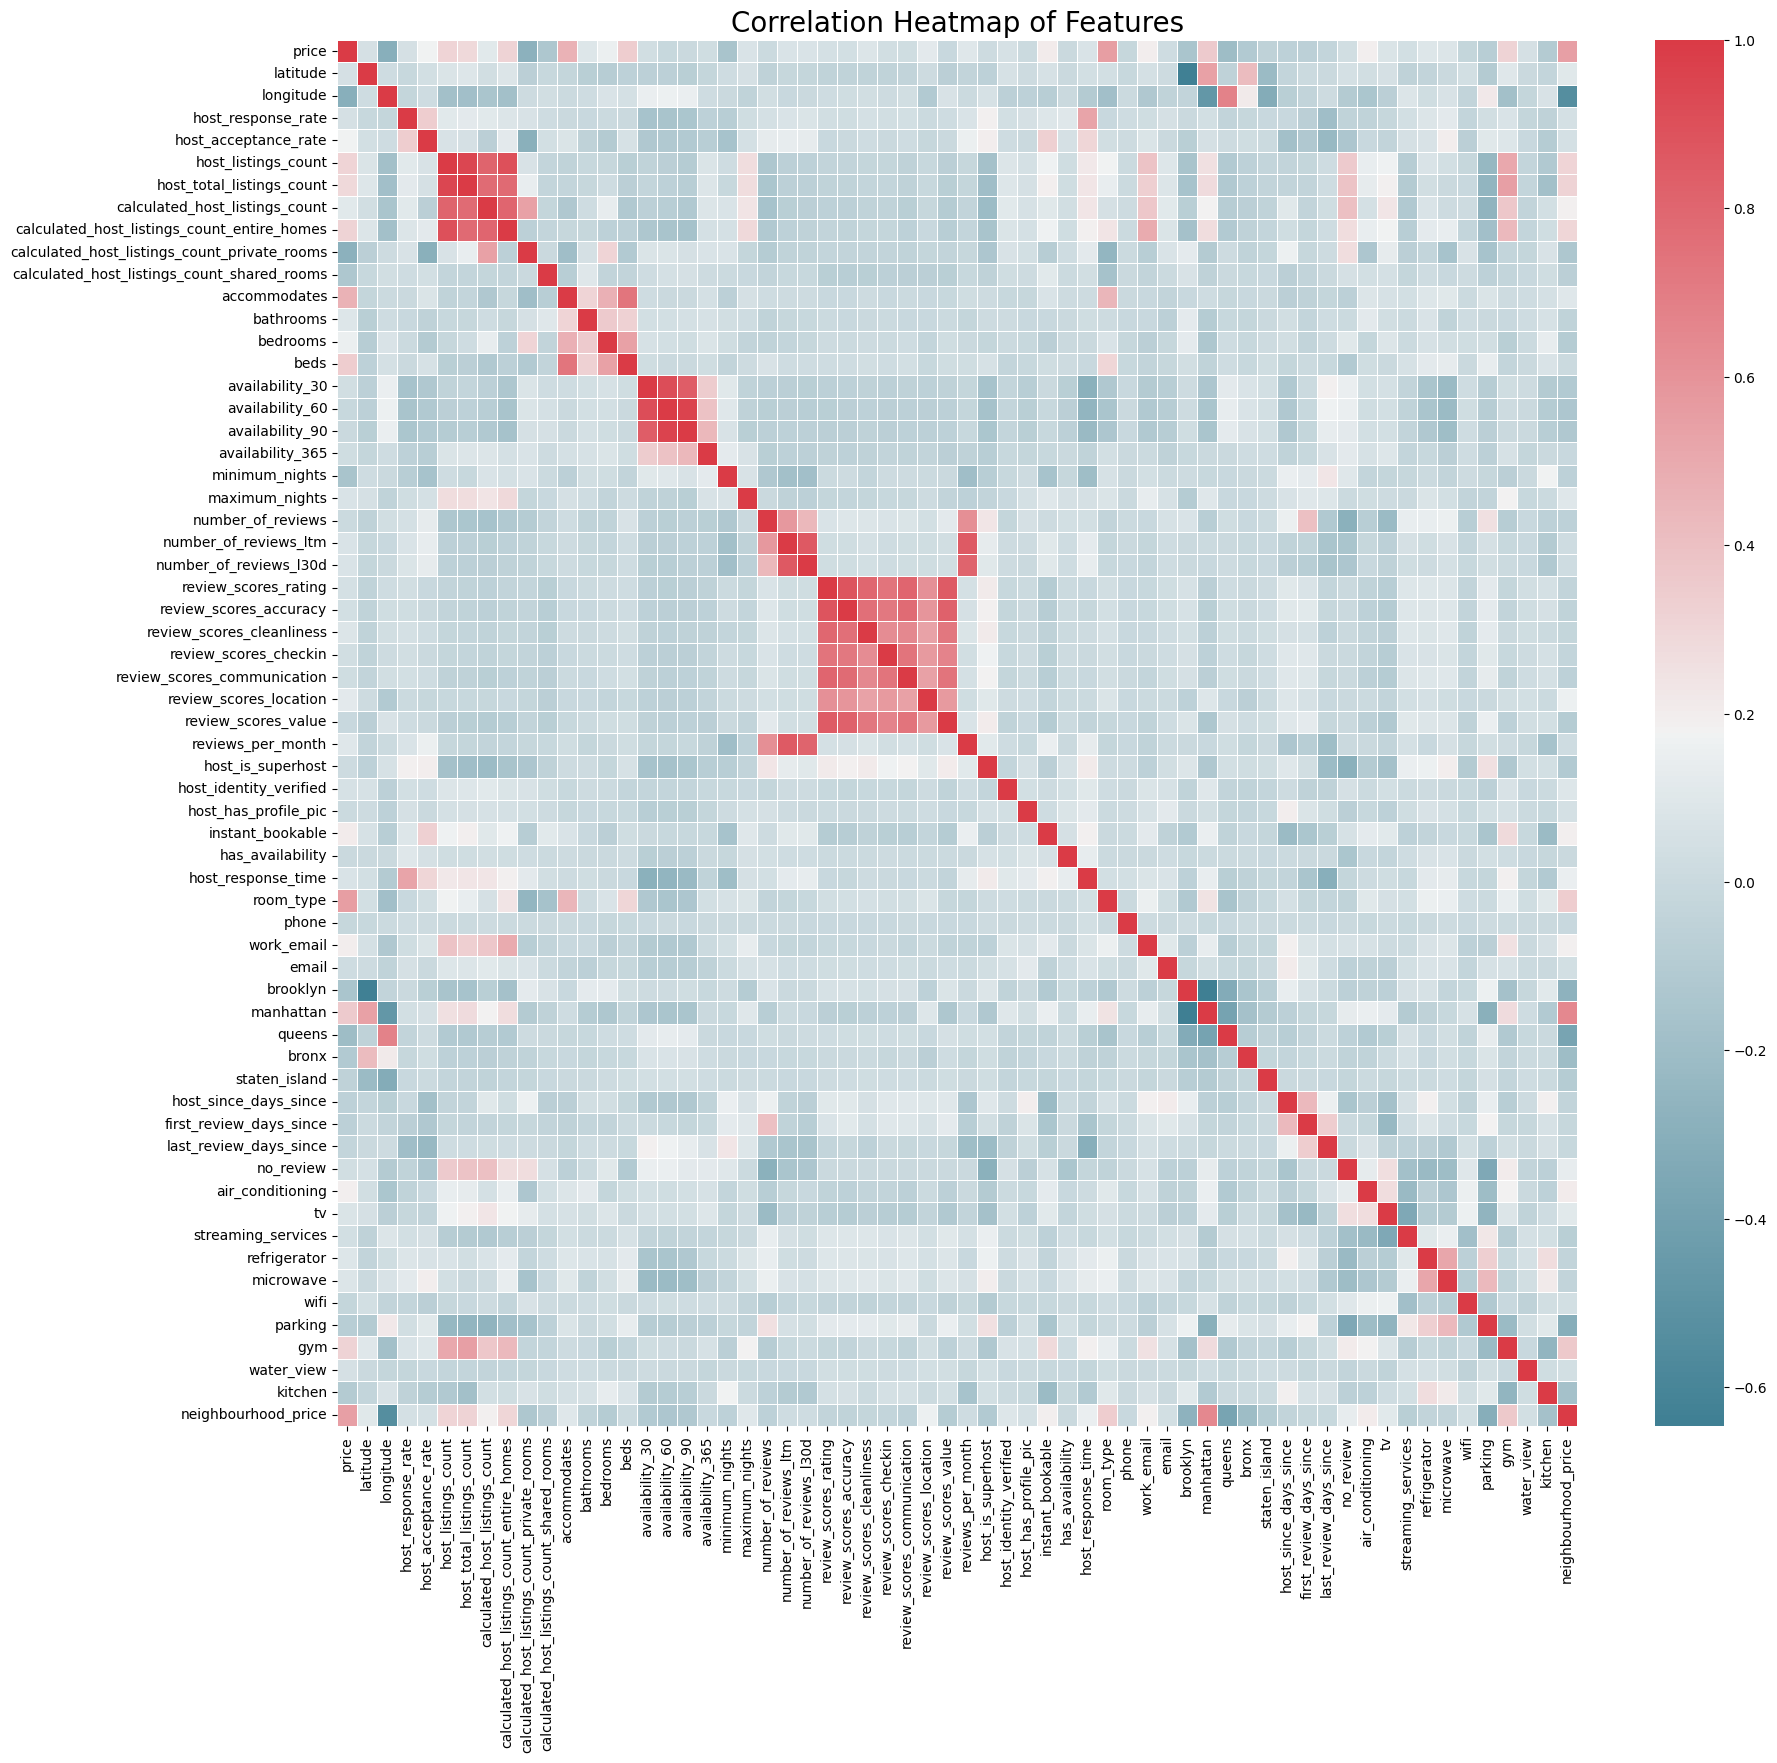
\includegraphics[width=0.8\textwidth]{images/correlation_before.png}
\caption{Correlation Heatmap Before PCA}
\label{fig:correlation_before}
\end{figure}

To reduce data complexity and improve model generalization, we applied PCA to the following feature groups, which showed high correlation in the previous matrix. Then, we generated all pairwise plots generated by each block, as shown in Figure \ref{fig:pairwise_plots}.

\begin{enumerate}
    \item \textbf{Availability Features:} \texttt{availability\_30}, \texttt{availability\_60}, and \texttt{availability\_90} were highly correlated (Figure \ref{fig:availability_short}) as they represent Airbnb availability in the next 30, 60, and 90 days, respectively. PCA reduced these to a single feature, \texttt{availability\_short}.
    
    \item \textbf{Host Listings Features:} \texttt{host\_listings\_count}, \texttt{host\_total\_listings\_count}, \texttt{calculated\_host\_listings\_count}, and \texttt{calculated\_host\_listings\_count\_entire\_homes} were highly correlated (Figure \ref{fig:hlc_short}), representing various aspects of the host's listing count. PCA reduced these to \texttt{hlc\_short}.
    
    \item \textbf{Number of Reviews Features:} \texttt{number\_of\_reviews}, \texttt{number\_of\_reviews\_ltm}, \texttt{number\_of\_reviews\_l30d}, and \texttt{reviews\_per\_month} were highly correlated (Figure \ref{fig:nor_short}), indicating overall review activity. PCA reduced these to \texttt{nor\_short}.
    
    \item \textbf{Review Scores Features:} \texttt{review\_scores\_rating}, \texttt{review\_scores\_accuracy}, \texttt{review\_scores\_cleanliness}, \texttt{review\_scores\_checkin}, \texttt{review\_scores\_communication}, \texttt{review\_scores\_location}, and \texttt{review\_scores\_value} were highly correlated (Figure \ref{fig:rs_short}), reflecting overall review quality. PCA reduced these to \texttt{rs\_short}.
\end{enumerate}

\begin{figure}[H]
\centering
\begin{subfigure}[b]{0.4\textwidth}
    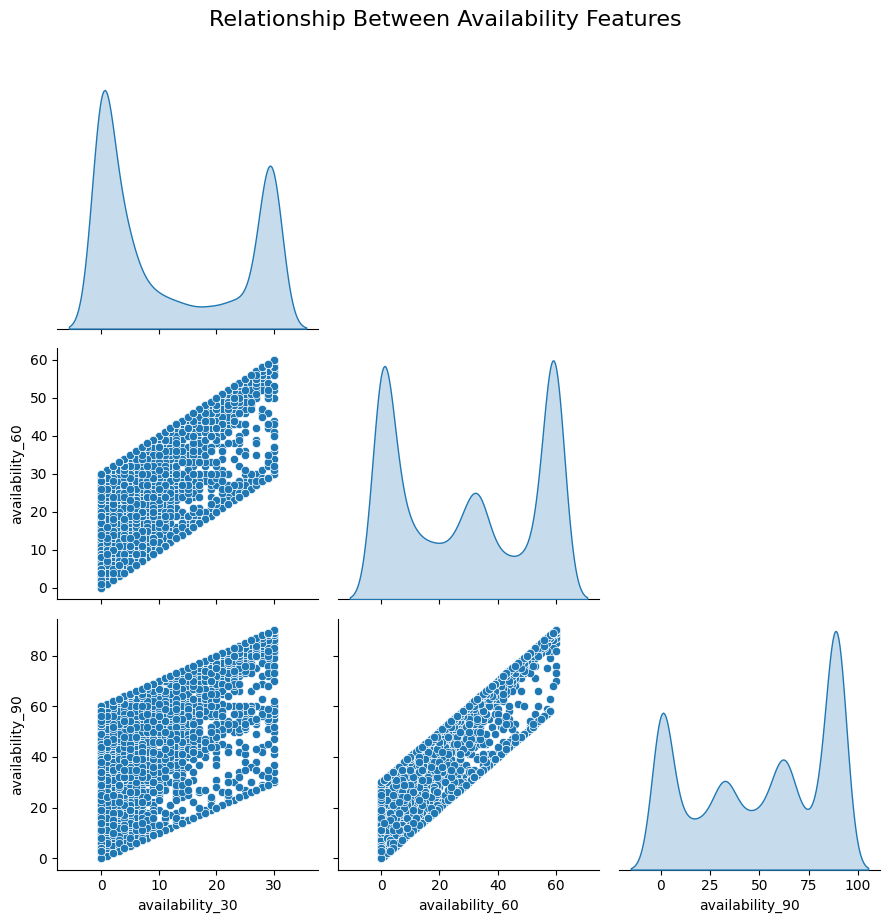
\includegraphics[width=\textwidth]{images/availability_short.png}
    \caption{Availability Features}
    \label{fig:availability_short}
\end{subfigure}
\hfill
\begin{subfigure}[b]{0.4\textwidth}
    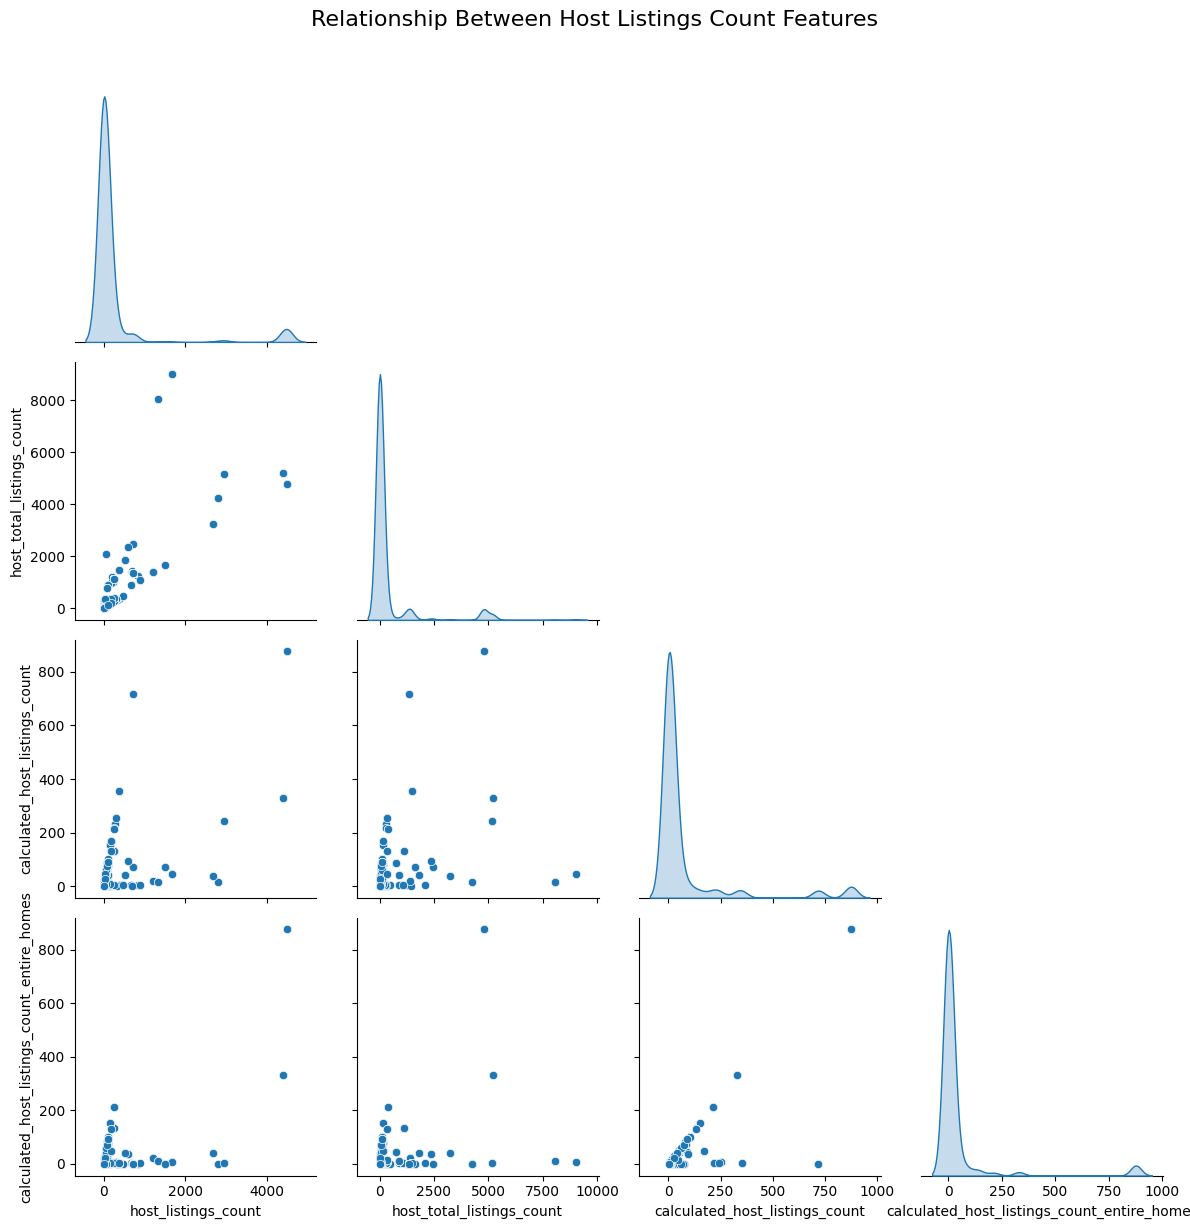
\includegraphics[width=\textwidth]{images/hlc_short.png}
    \caption{Host Listings Features}
    \label{fig:hlc_short}
\end{subfigure}

\begin{subfigure}[b]{0.4\textwidth}
    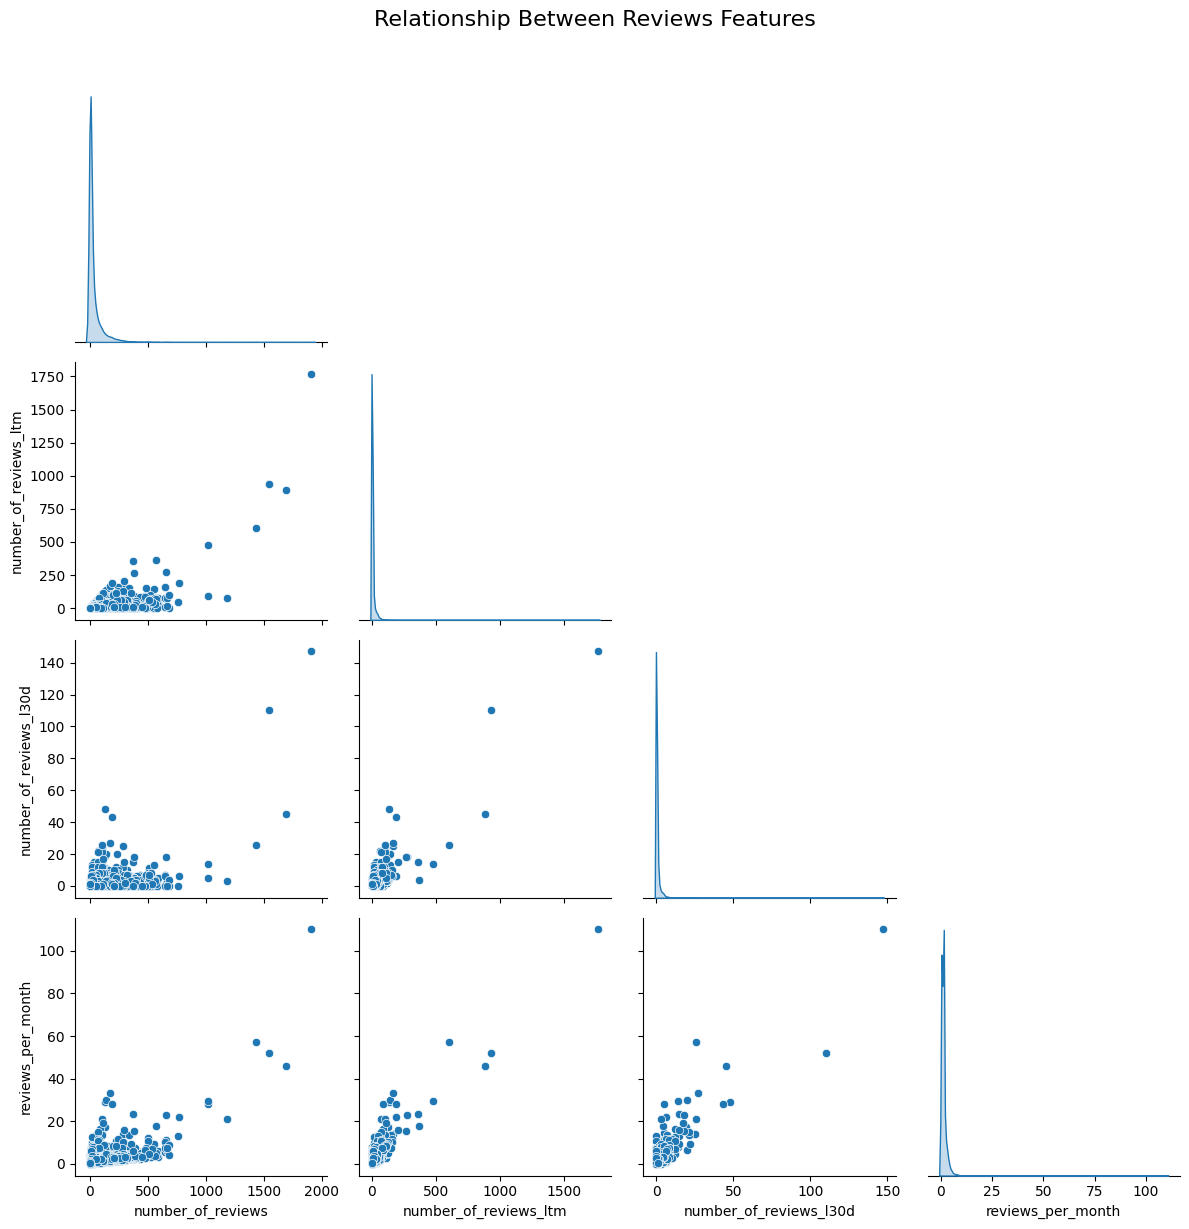
\includegraphics[width=\textwidth]{images/nor_short.png}
    \caption{Number of Reviews Features}
    \label{fig:nor_short}
\end{subfigure}
\hfill
\begin{subfigure}[b]{0.4\textwidth}
    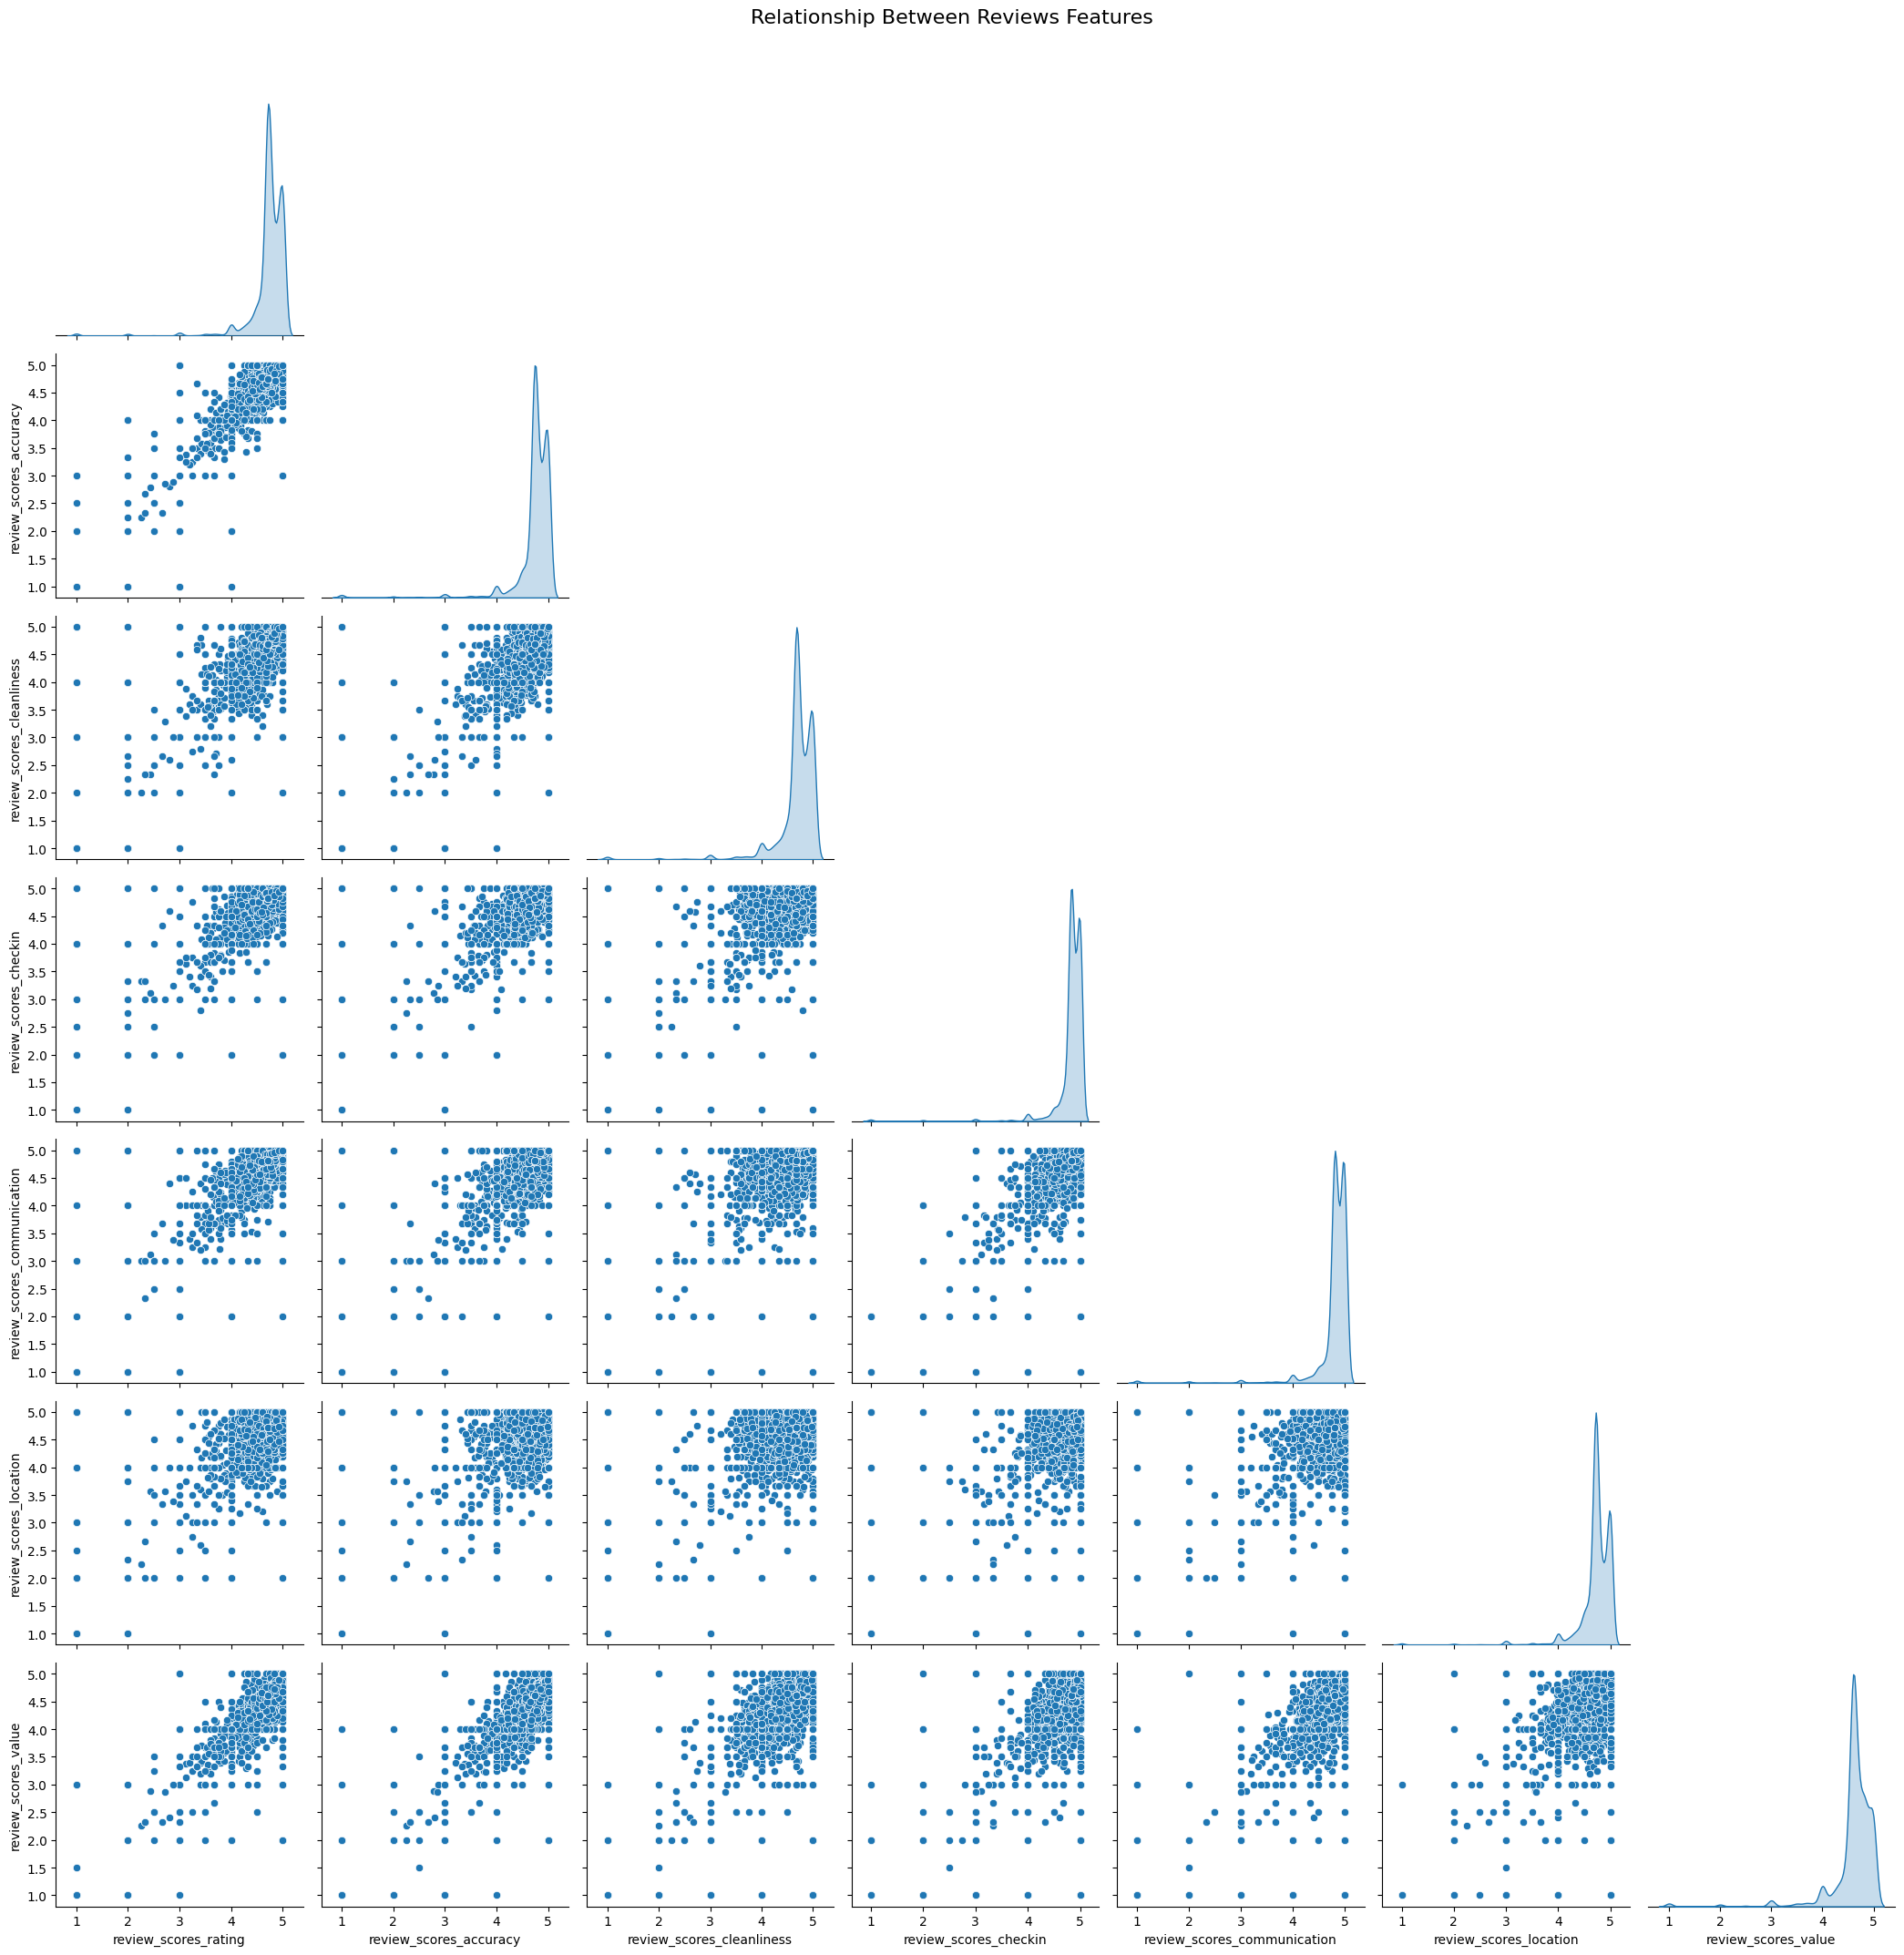
\includegraphics[width=\textwidth]{images/rs_short.png}
    \caption{Review Scores Features}
    \label{fig:rs_short}
\end{subfigure}
\caption{Pairwise Relationships of Feature Groups}
\label{fig:pairwise_plots}
\end{figure}

After applying PCA and dropping the original correlated variables, the correlation heatmap (Figure \ref{fig:correlation_after}) shows a reduction in multicollinearity, facilitating better model generalization and reduced data complexity.

\begin{figure}[H]
\centering
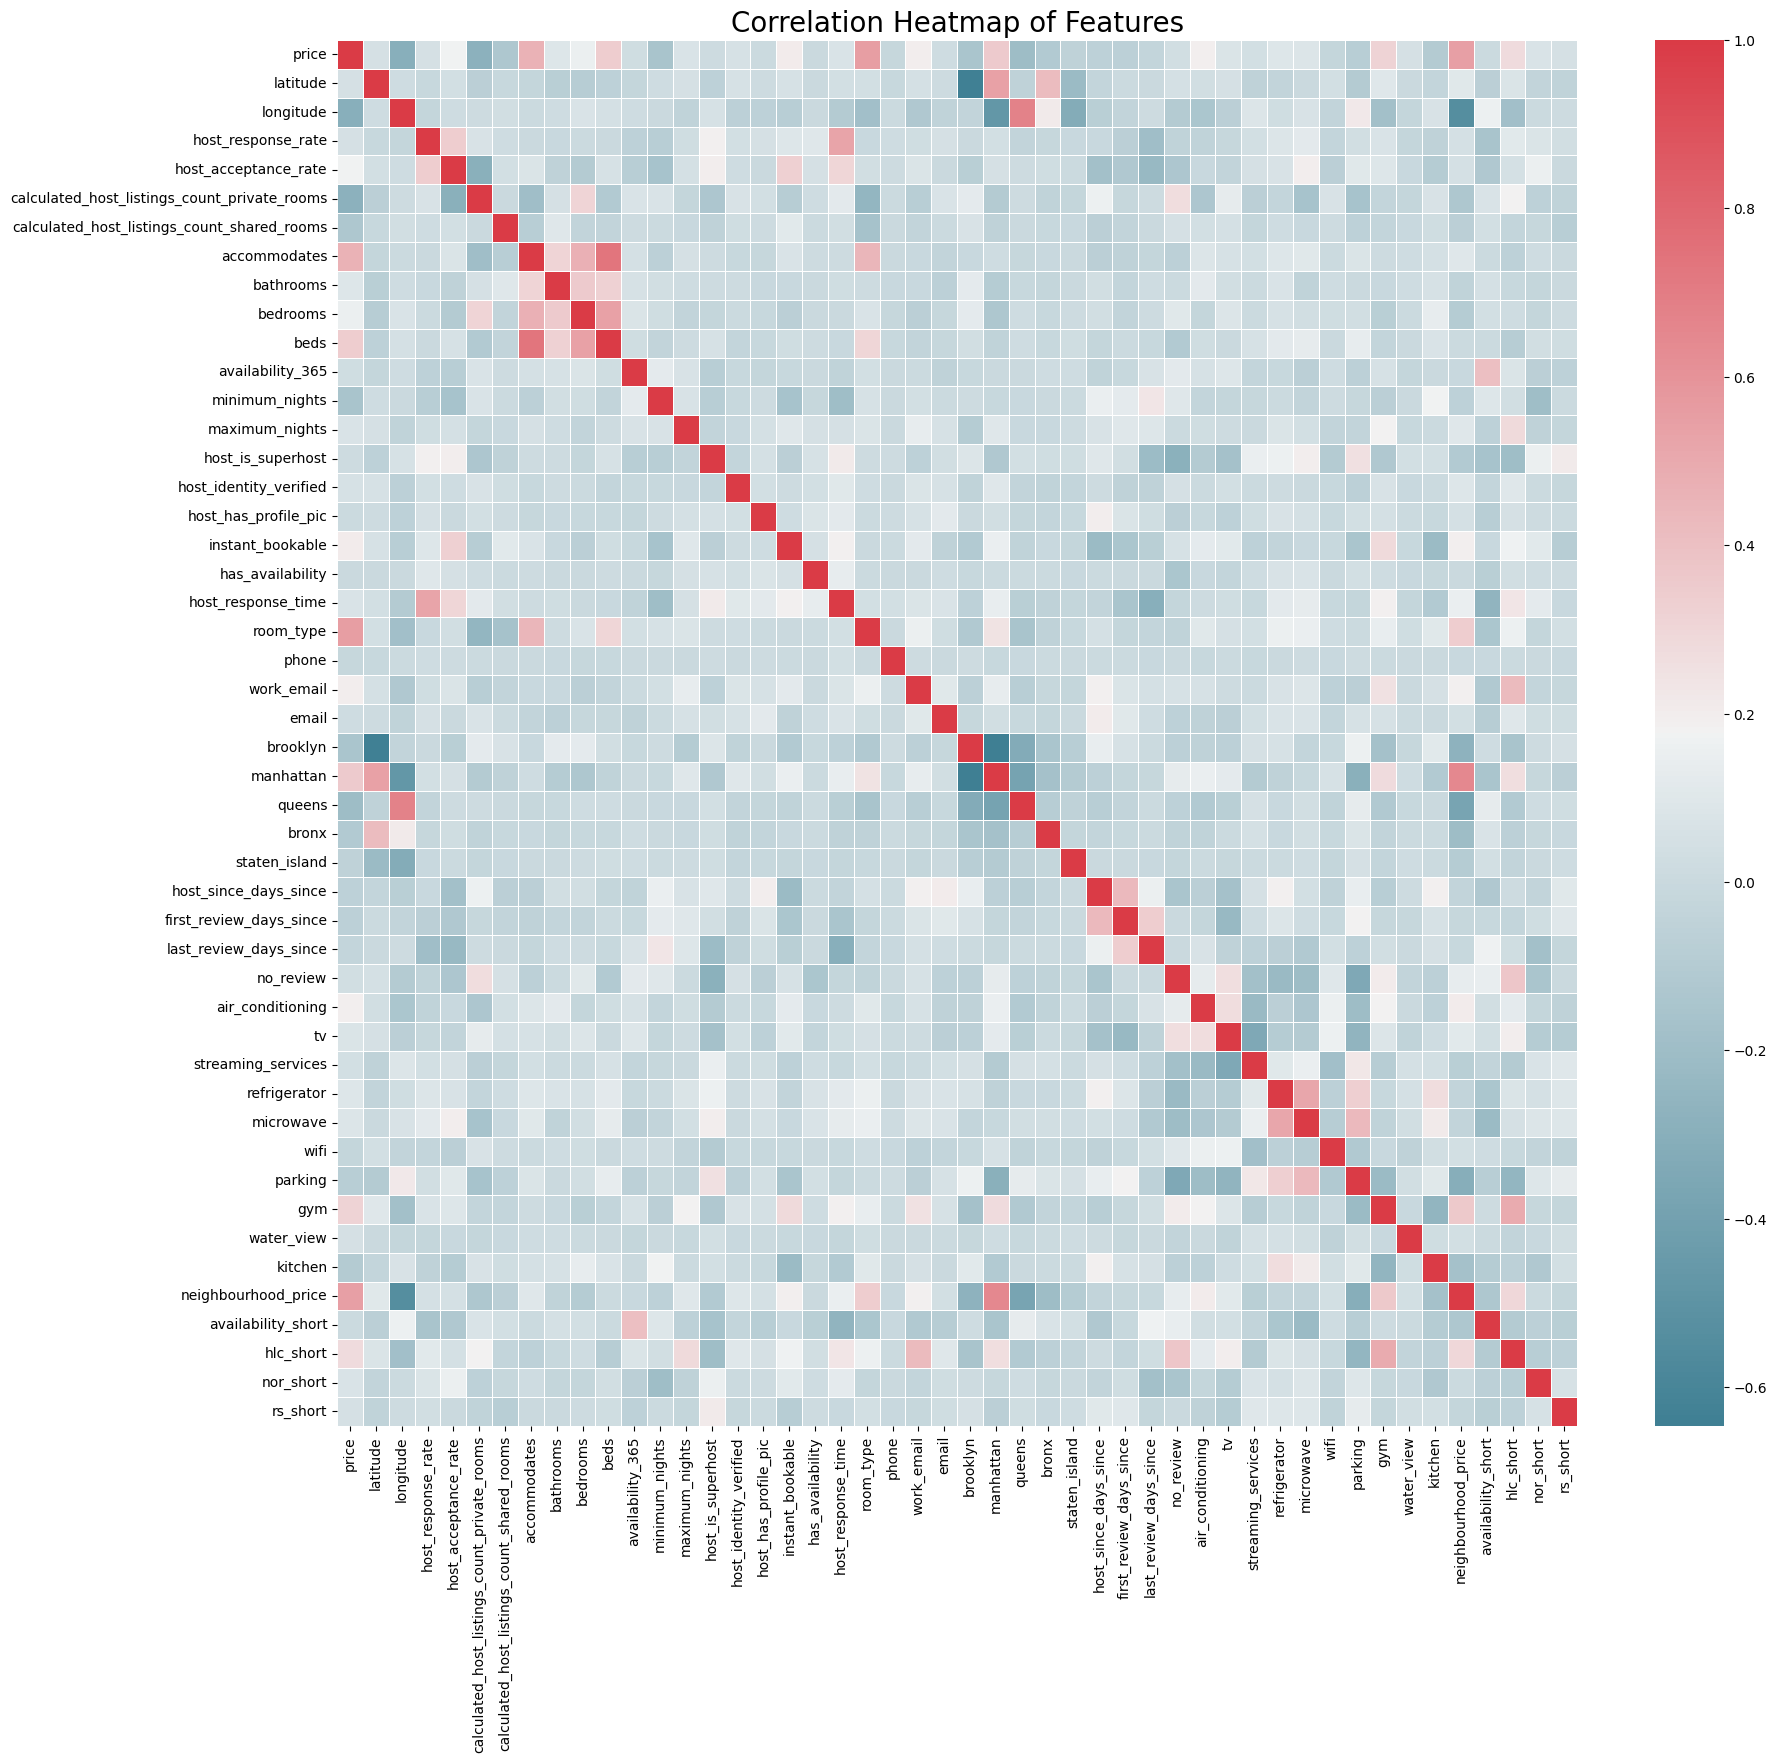
\includegraphics[width=0.8\textwidth]{images/correlation_after.png}
\caption{Correlation Heatmap After PCA}
\label{fig:correlation_after}
\end{figure}

\subsection{Outliers and Distribution Normalization}

We examined the distribution of each feature at this point to identify outliers and non-standard distributions that could impact model performance. Figures \ref{fig:df_describe} and \ref{fig:df_distribution} show the summary statistics and distributions of the features, respectively.

\begin{figure}[H]
\centering
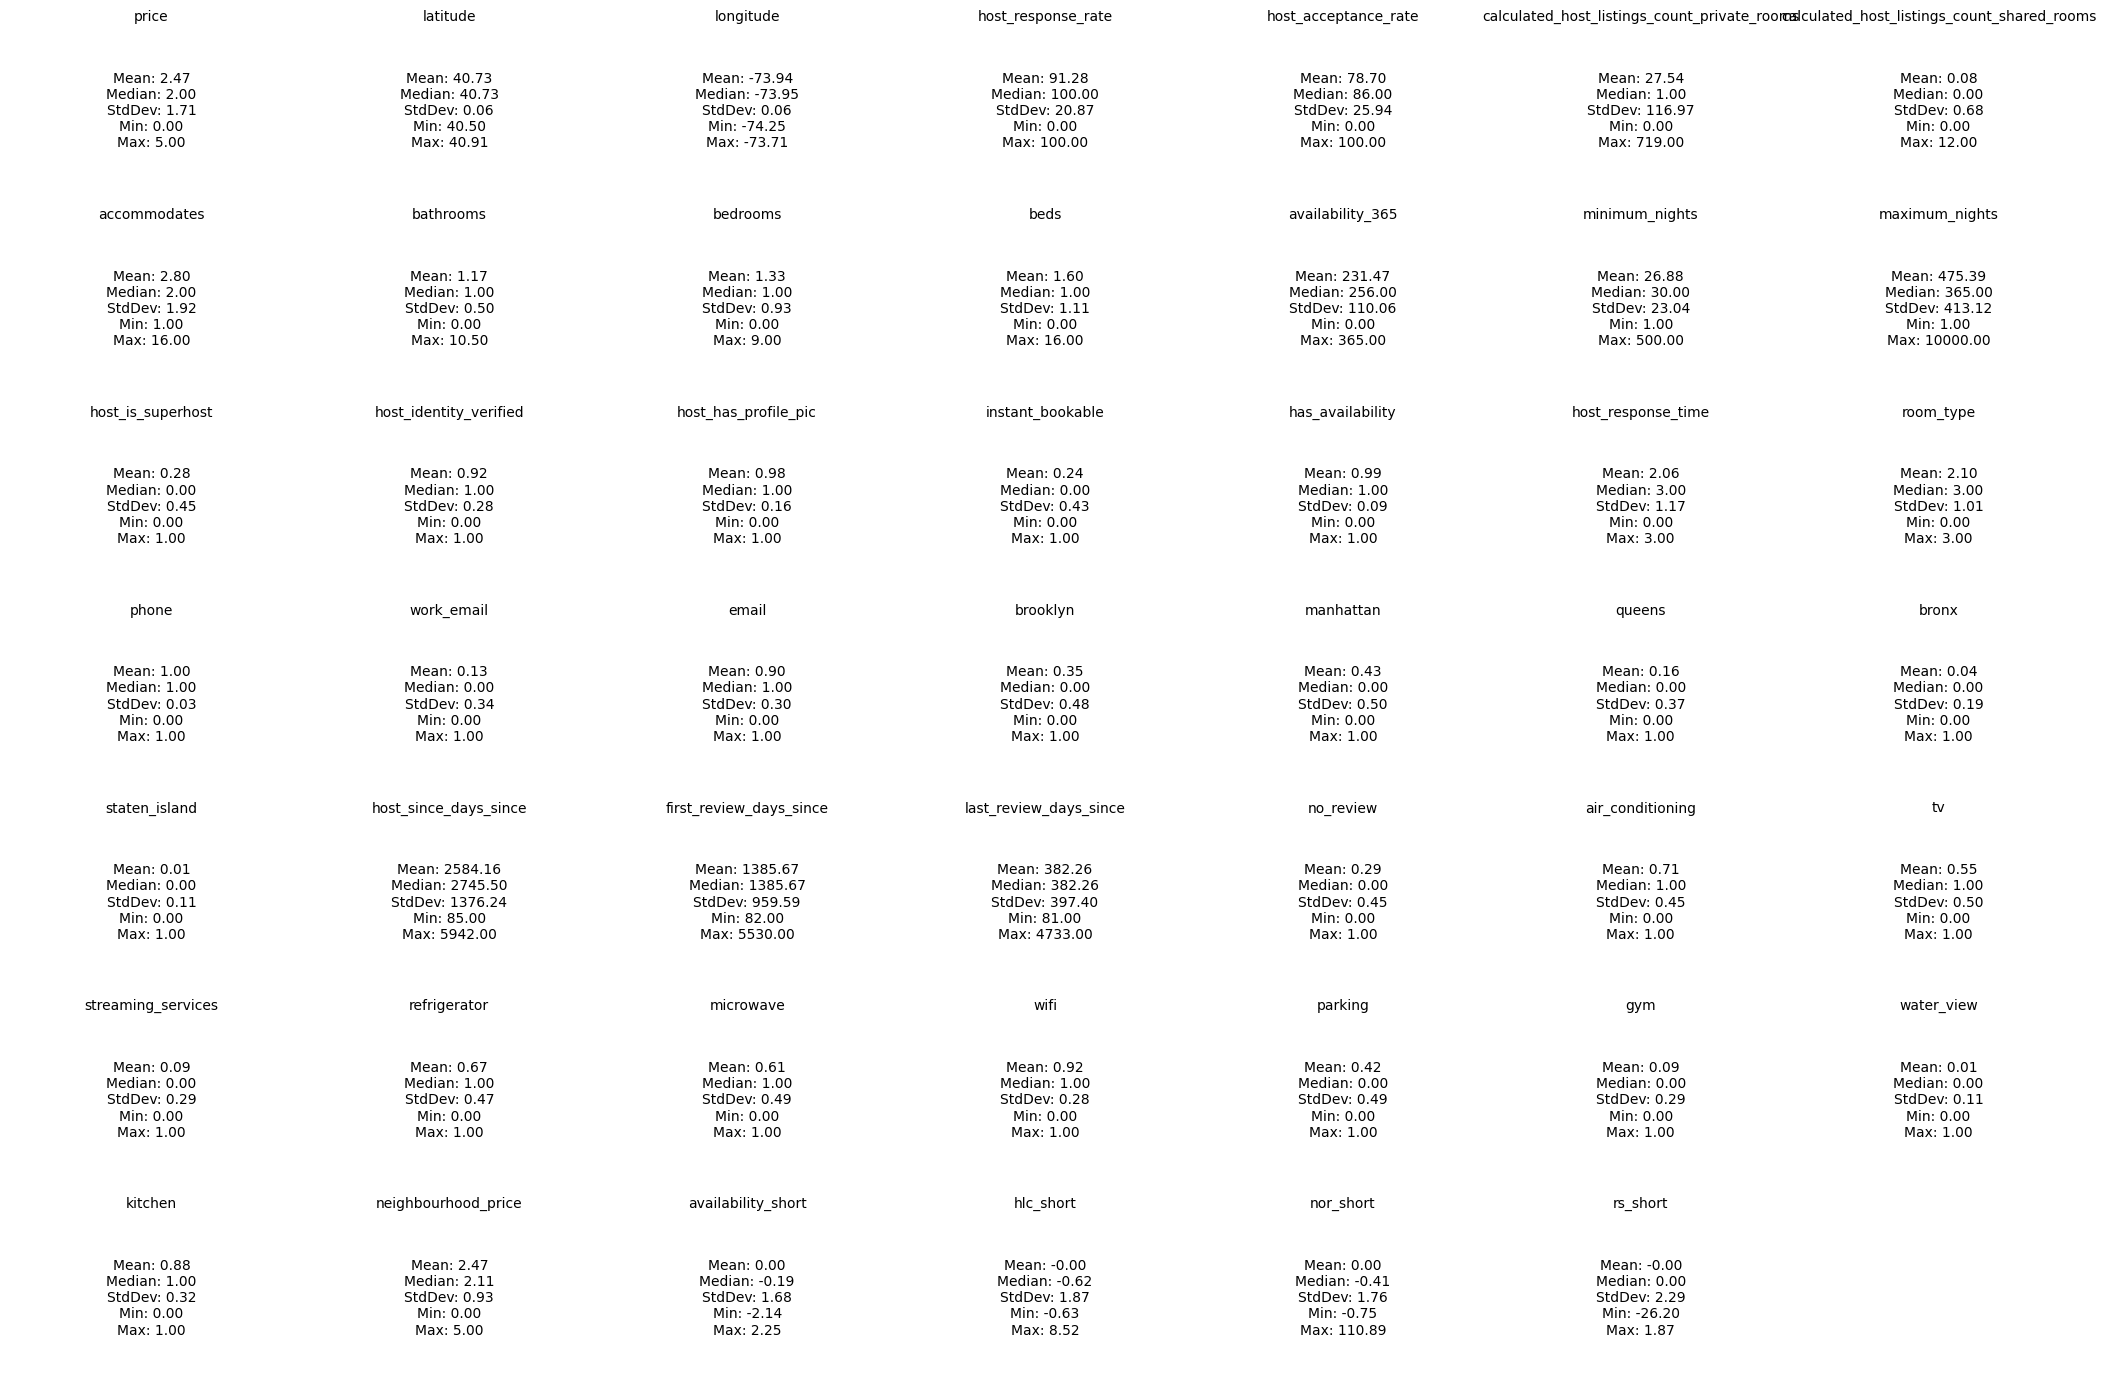
\includegraphics[width=0.65\textwidth]{images/df_describe.png}
\caption{Summary Statistics of Features}
\label{fig:df_describe}
\end{figure}

\begin{figure}[H]
\centering
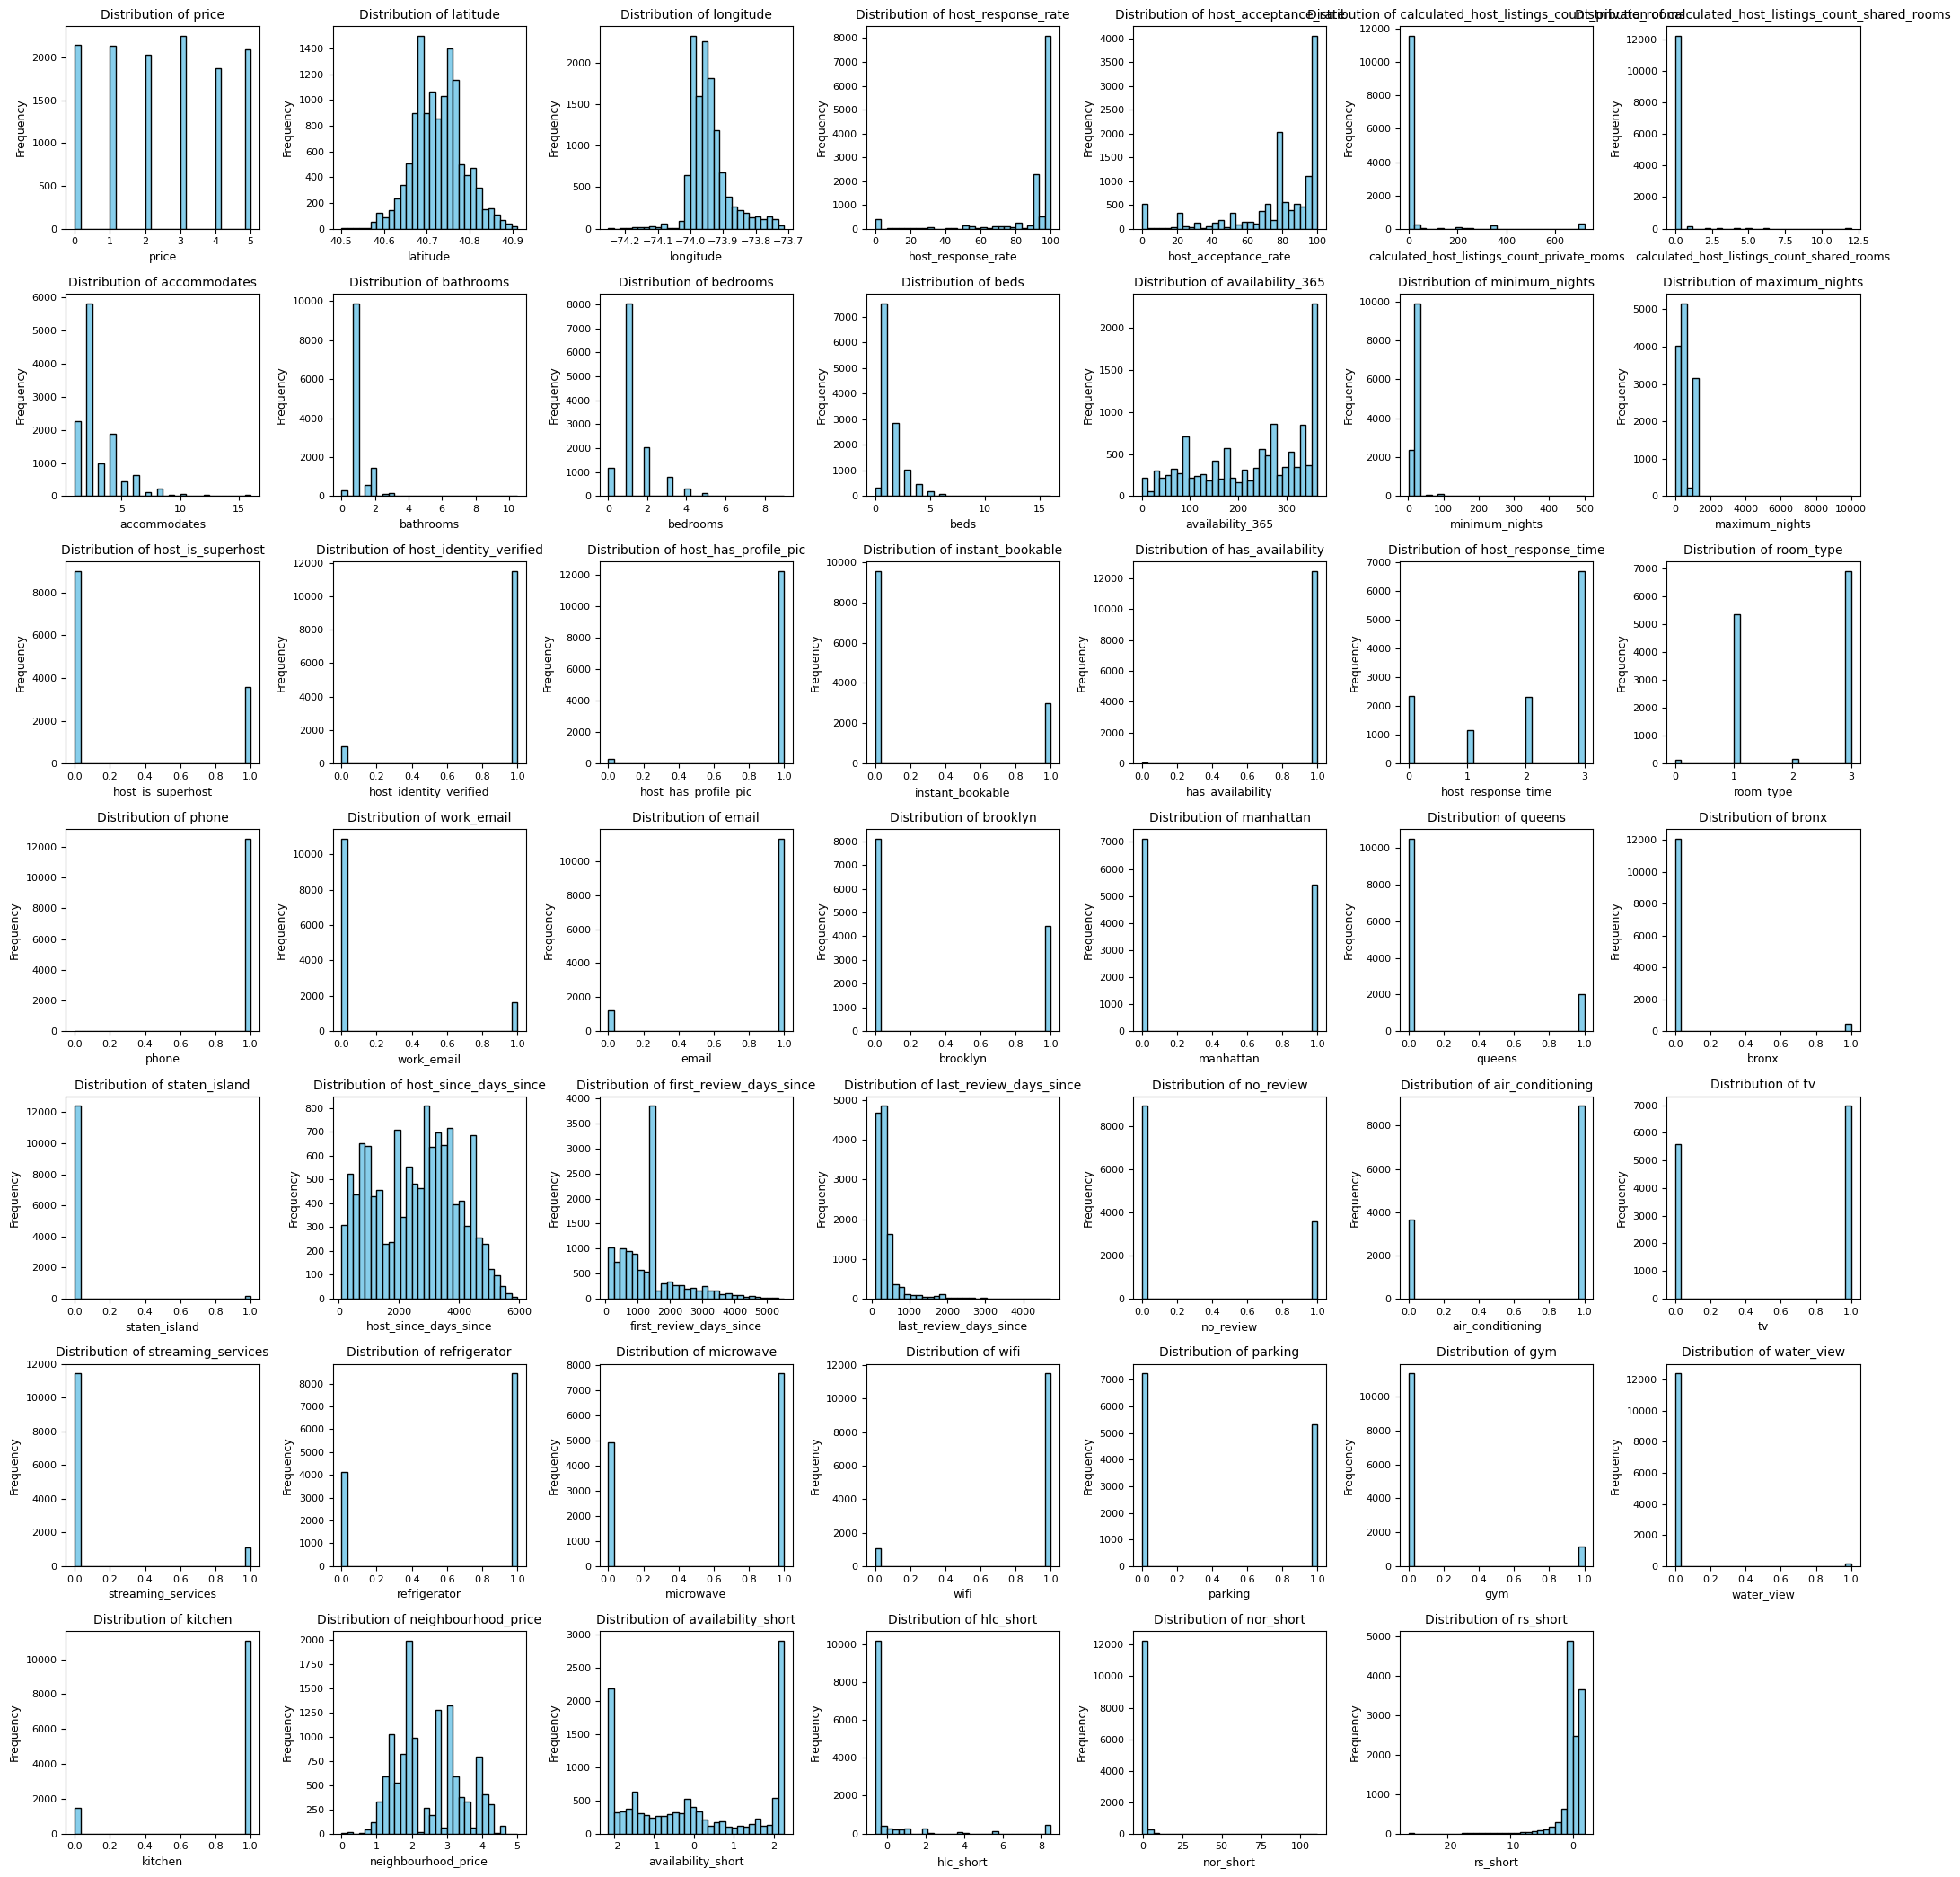
\includegraphics[width=0.65\textwidth]{images/df_distribution.png}
\caption{Distribution of Features}
\label{fig:df_distribution}
\end{figure}
    

\subsubsection{\texttt{calculated\_host\_listings\_count\_private\_rooms}}

\begin{figure}[H]
\centering
\begin{subfigure}[b]{0.48\textwidth}
    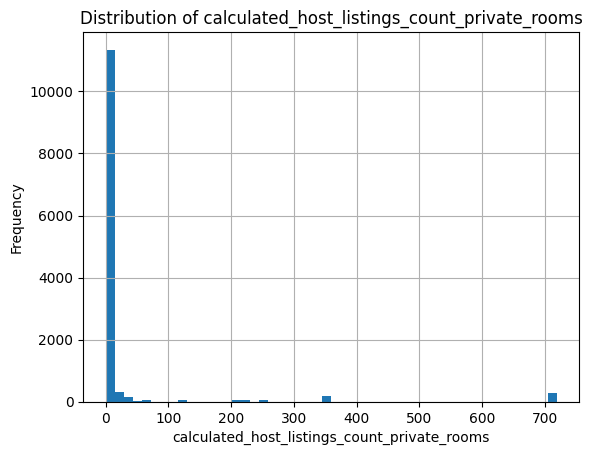
\includegraphics[width=\textwidth]{images/private_rooms_before.png}
    \caption{Before Processing}
    \label{fig:hlcpr_before}
\end{subfigure}
\hfill
\begin{subfigure}[b]{0.48\textwidth}
    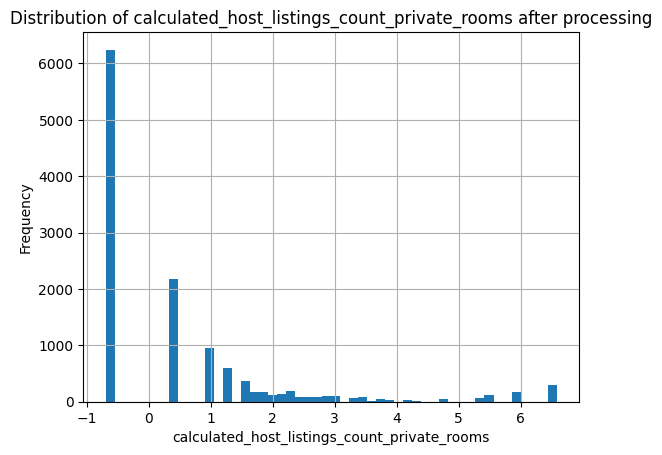
\includegraphics[width=\textwidth]{images/private_rooms_after.png}
    \caption{After Processing}
    \label{fig:hlcpr_after}
\end{subfigure}
\caption{Distribution of \texttt{calculated\_host\_listings\_count\_private\_rooms}}
\end{figure}

The feature \texttt{calculated\_host\_listings\_count\_private\_rooms} exhibited an exponential-like distribution. Hence, we applied the logarithmic transformation:

\[
x \to \log(x + 0.5)
\]

Adding 0.5 avoids taking the logarithm of zero and ensures that a value of 0 maps close to 1. This transformation normalizes the distribution, making it more suitable for machine learning models. However, since decision tree-based models like Random Forests and XGBoost are insensitive to monotonic transformations, this change did not impact their performance. Conversely, for models like Logistic Regression, the transformation improved performance.

The distribution before this transformation is shown in Figure \ref{fig:hlcpr_before}, while the distribution after the transformation is shown in Figure \ref{fig:hlcpr_after}.

\subsubsection{\texttt{minimum\_nights} and \texttt{maximum\_nights}}

\begin{figure}[H]
\centering
\begin{subfigure}[b]{0.48\textwidth}
    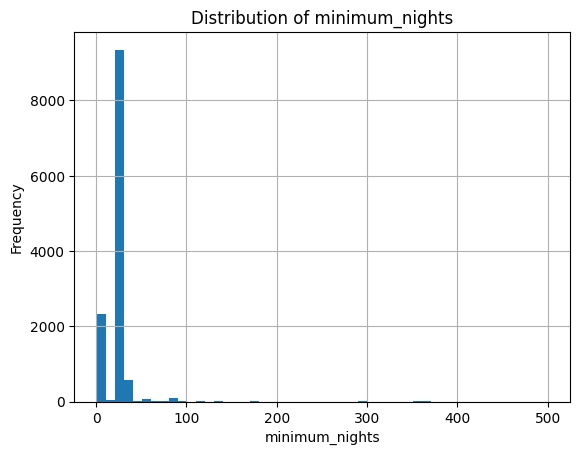
\includegraphics[width=\textwidth]{images/minimum_nights_before.png}
    \caption{Minimum Nights Before Processing}
    \label{fig:min_nights_before}
\end{subfigure}
\hfill
\begin{subfigure}[b]{0.48\textwidth}
    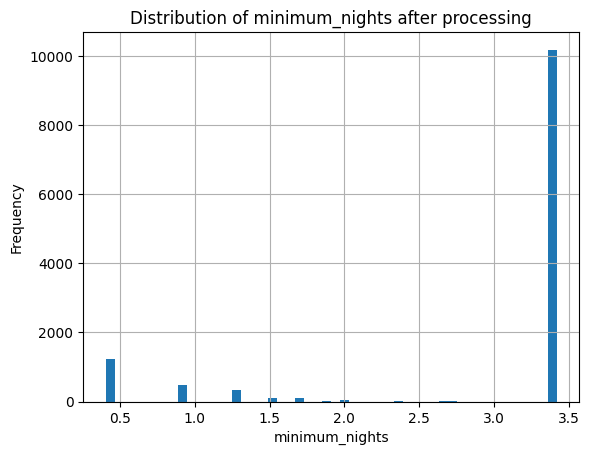
\includegraphics[width=\textwidth]{images/minimum_nights_after.png}
    \caption{Minimum Nights After Processing}
    \label{fig:min_nights_after}
\end{subfigure}

\begin{subfigure}[b]{0.48\textwidth}
    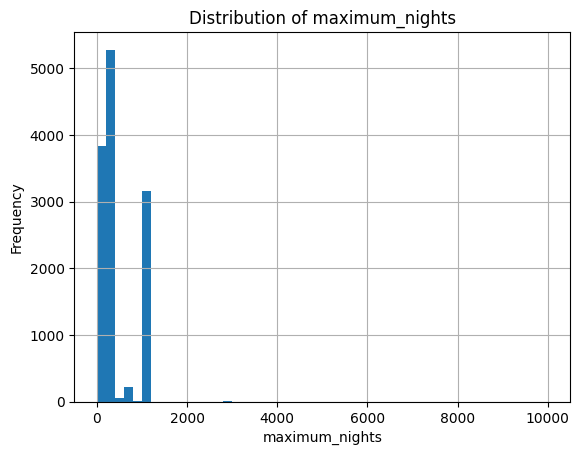
\includegraphics[width=\textwidth]{images/maximum_nights_before.png}
    \caption{Maximum Nights Before Processing}
    \label{fig:max_nights_before}
\end{subfigure}
\hfill
\begin{subfigure}[b]{0.48\textwidth}
    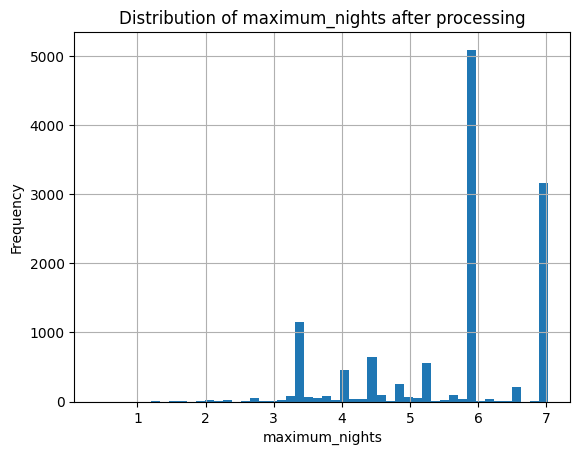
\includegraphics[width=\textwidth]{images/maximum_nights_after.png}
    \caption{Maximum Nights After Processing}
    \label{fig:max_nights_after}
\end{subfigure}
\caption{Distributions of \texttt{minimum\_nights} and \texttt{maximum\_nights}}
\end{figure}

We observed outliers in \texttt{minimum\_nights} and \texttt{maximum\_nights}. To address this:

\begin{itemize}
    \item For \texttt{minimum\_nights}, we capped values above 30 to 30, as the 99th percentile was 30. This decision was based on the rationale that requiring more than 30 nights is uncommon and likely represents long-term rentals, which should be treated uniformly.
    
    \item For \texttt{maximum\_nights}, we capped values above 1,124 to 1,124, as this represented an extreme outlier (approximately 4 years). This capping prevents undue influence from these rare cases.
    
    \item As both distributions exhibited exponential-like behavior, we transformed both features using:
    \[
    x \to \log(x + 0.5)
    \]
\end{itemize}

The distributions before these transformations are shown in Figures \ref{fig:min_nights_before} and \ref{fig:max_nights_before}, while the distributions after the transformations are shown in Figures \ref{fig:min_nights_after} and \ref{fig:max_nights_after}.

\subsection{Feature Dropping}

We excluded the following features due to minimal informational value:

\begin{itemize}
    \item \texttt{calculated\_host\_listings\_count\_shared\_rooms}
    \item \texttt{has\_availability}
    \item \texttt{work\_email}
\end{itemize}

\subsection{Feature Engineering}

To enhance model interpretability, we created new features:

\begin{itemize}
    \item \textbf{Amenities Count:} Defined as the sum of all one-hot encoded amenity features.
    \[
    \begin{aligned}
    \texttt{amenities\_count} =\ & \texttt{air\_conditioning} + \texttt{tv} + \texttt{streaming\_services} \\
    & + \texttt{refrigerator} + \texttt{microwave} + \texttt{wifi} \\
    & + \texttt{parking} + \texttt{gym} + \texttt{water\_view} + \texttt{kitchen}
    \end{aligned}
    \]        
    This aggregated count allows decision trees to evaluate the number of amenities more efficiently, without incurring a regularization penalty.
    
    \item \textbf{Host Responsiveness:} Defined as the product of \texttt{host\_response\_time} and \texttt{host\_response\_rate}.
    \[
    \texttt{host\_responsiveness} = \texttt{host\_response\_time} \times \texttt{host\_response\_rate}
    \]
    This composite score ranges from 0 to 300, representing overall host responsiveness after normalization.
\end{itemize}

\section{Models}

In this project, we employed two different algorithms for generating predictions: Random Forests and XGBoost. The selection of these models was motivated by their ability to handle complex datasets with numerous features, their robustness to overfitting, and the availability of high-quality implementations in popular machine learning libraries.

Initially, we experimented with various classification and regression models, including Linear Regression, Logistic Regression, Decision Trees, and Neural Networks. However, these models did not yield satisfactory performance on the dataset.

\subsection{Ineffective Models}

Linear Regression and Logistic Regression were not complex enough to capture the intricate relationships within the data. With approximately 50 features, these models struggled to model the non-linear interactions between variables effectively. This limitation was evident as both training and validation RMSE scores were high and similar, indicating underfitting.

Decision Trees, while capable of modeling non-linear patterns, tended to overfit the training data when not properly regularized. Even with techniques like pruning, individual decision trees did not perform well due to the high dimensionality and complexity of the dataset.

Neural Networks are powerful models known for their ability to learn complex patterns. However, they typically require large amounts of data to perform optimally. In this case, the dataset contained around 15,000 data points, which was insufficient for training an effective neural network without encountering overfitting or underfitting issues. Additionally, neural networks are computationally intensive and require careful tuning of numerous hyperparameters, which was not practical.

\subsection{Rationale Behind Model Selection}

A common motivation for both models is feature importance: both Random Forests and XGBoost provide tools for feature importance analysis, enabling a better understanding of the models' decision-making processes.

\subsubsection{Random Forest}

Random Forest is an ensemble learning method that constructs multiple decision trees during training and outputs the mean prediction of the individual trees. This approach reduces variance and mitigates overfitting by averaging out the biases of individual trees.

A key motivation for choosing Random Forests is their computational efficiency. While more complex than individual decision trees, Random Forests are parallelizable and computationally efficient, making them suitable for datasets of this size.

\subsubsection{XGBoost}

XGBoost (Extreme Gradient Boosting) is an optimized gradient boosting framework that uses tree-based models. It builds models sequentially, where each new tree focuses on correcting the errors of the previous ones.

Key motivations for choosing XGBoost include flexibility and efficiency. XGBoost offers extensive hyperparameter tuning options to optimize model performance, making it suitable for complex datasets. Additionally, XGBoost is designed for speed and performance, handling large datasets efficiently.

\subsection{Rationale for Regression Models}

We employed the \texttt{XGBRegressor} from the \texttt{xgboost} library, which offers an efficient and scalable implementation of the algorithm, and the \texttt{RandomForestRegressor} from \texttt{scikit-learn}, a robust implementation of Random Forests.

Although this project was framed as a classification problem, we discovered that using regression models and rounding their outputs provided better results than the classification versions of these models. By leveraging the regression capabilities of XGBoost and applying post-processing techniques, we were able to enhance the predictive performance, achieving more accurate and reliable outcomes.

\subsection{External Libraries}

Both models were implemented using \texttt{scikit-learn} and \texttt{xgboost}, which provide robust implementations of Random Forests and XGBoost, respectively. These libraries are open-source and widely used in the machine learning community and offer extensive functionality for model training, evaluation, and hyperparameter tuning.

\section{Hyperparameter Selection}

To achieve optimal performance for both the \texttt{XGBRegressor} and \texttt{RandomForestRegressor} models, careful tuning of hyperparameters was essential. Hyperparameters, such as the number of trees in a Random Forest or the learning rate in XGBoost, significantly influence model performance. Selecting appropriate hyperparameter values ensures that the models generalize well to unseen data without overfitting.

\subsection{Optuna for Hyperparameter Optimization}

We utilized Optuna, a hyperparameter optimization framework in Python, to automate the search for optimal hyperparameter configurations. Optuna employs Bayesian Optimization, specifically using the Tree-structured Parzen Estimator (TPE) as its surrogate model. This method models the objective function $f(\mathbf{x})$, where $\mathbf{x}$ represents the hyperparameters, by estimating two probability densities:
\[
l(\mathbf{x}) = p(\mathbf{x} \mid f(\mathbf{x}) < y^*)
\]
for promising hyperparameters and
\[
g(\mathbf{x}) = p(\mathbf{x})
\]
for all possible hyperparameters. The TPE approach optimizes the selection of the next set of hyperparameters by maximizing the ratio:
\[
\frac{l(\mathbf{x})}{g(\mathbf{x})}
\]
This ratio prioritizes hyperparameters that are more likely to yield better performance based on past evaluations, effectively balancing exploration and exploitation in the search space.

\subsection{Hyperparameter Optimization Process}

\subsubsection{XGBoost Regressor}

For the \texttt{XGBRegressor}, the hyperparameter optimization involved tuning parameters such as the learning rate ($\eta$), maximum tree depth ($d$), and the number of estimators ($n$). We also optimized hyperparameters like \texttt{subsample}, \texttt{colsample\_bytree}, \texttt{gamma}, \texttt{min\_child\_weight}, \texttt{reg\_alpha}, and \texttt{reg\_lambda}.

Initially, we conducted a preliminary search with a narrow range of hyperparameters, which allowed us to train a reasonably good model in approximately 10 minutes on our computer. This initial model provided a baseline for performance.

To further enhance the model's accuracy, we extended the search by allowing Optuna to explore a wider range of hyperparameters over a duration of 4 hours. This extensive search enabled the identification of the best-performing hyperparameter configuration, which significantly improved the model's predictive capabilities.

\subsubsection{Random Forest Regressor}

Similarly, for the \texttt{RandomForestRegressor}, hyperparameter tuning was crucial due to the model's inherent complexity and sensitivity to parameter settings. Key hyperparameters included the number of trees (\texttt{n\_estimators}), maximum tree depth (\texttt{max\_depth}), and the minimum number of samples required to split an internal node (\texttt{min\_samples\_split}). We also optimized hyperparameters like \texttt{min\_samples\_leaf}, \texttt{max\_features}, and \texttt{bootstrap}.

Given that training a single Random Forest model is computationally more intensive than XGBoost, the hyperparameter optimization process for Random Forests was more time-consuming. Optuna was run for 6 hours, allowing it to thoroughly explore the hyperparameter space and identify the optimal configuration that minimized the RMSE on the validation set.

\subsection{Advantages of Using Optuna}

The hyperparameter optimization was implemented using Optuna's \texttt{study.optimize} function, which iteratively evaluates different hyperparameter configurations based on the defined objective function.

Optuna is highly effective in optimizing hyperparameters due to its ability to handle a vast search space efficiently. Compared to manual hyperparameter tuning or simpler search methods like grid search, Optuna's Bayesian Optimization approach with TPE significantly outperformed in both speed and the quality of the resulting models. By automatically focusing on the most promising regions of the hyperparameter space, Optuna reduced the computational resources required and accelerated the discovery of optimal hyperparameter settings.

\subsection{Plotting}

To illustrate the impact of hyperparameter variations on model performance, we generated plots showing the relationship between specific hyperparameters and the RMSE on a subset of the training data.

\begin{figure}[H]
\centering
\begin{subfigure}[b]{0.48\textwidth}
    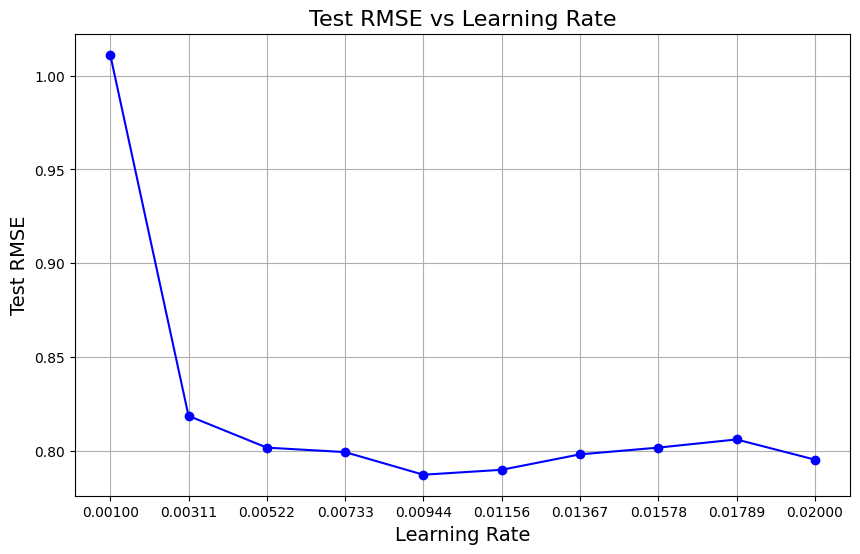
\includegraphics[width=\textwidth]{images/xgb_plot.png}
    \caption{XGB Learning Rate vs. RMSE}
    \label{fig:xgb_plot}
\end{subfigure}
\hfill
\begin{subfigure}[b]{0.48\textwidth}
    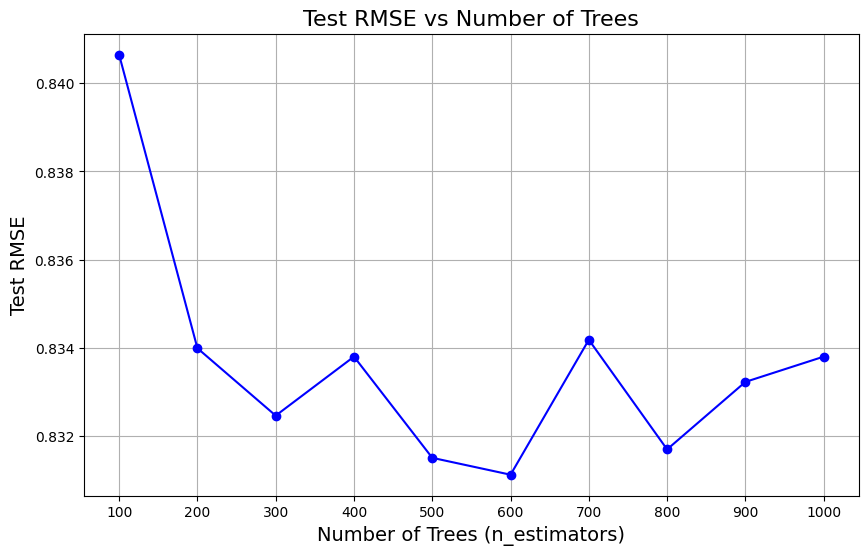
\includegraphics[width=\textwidth]{images/rf_plot.png}
    \caption{RF Number of Trees vs. RMSE}
    \label{fig:rf_plot}
\end{subfigure}
\caption{Hyperparameter Tuning Plots}
\label{fig:hyperparameter_tuning}
\end{figure}

Figure \ref{fig:xgb_plot} depicts how different learning rates ($\eta$) affect the RMSE of the \texttt{XGBRegressor}. This plot helped identify the optimal learning rate that minimized the RMSE on the validation set. Similarly, Figure \ref{fig:rf_plot} illustrates the effect of varying the number of trees (\texttt{n\_estimators}) in the \texttt{RandomForestRegressor} on the RMSE. This plot helped identify the optimal number of trees that minimized the RMSE on the validation set.

\section{Data Splits}

To ensure robust model evaluation and prevent overfitting, we split the dataset as follows:

\begin{itemize}
    \item The original \texttt{train.csv} dataset, referred to as the final train set, was deterministically split into an 80\% training subset and a 20\% validation subset. This allowed us to train the models on a majority of the data while retaining a separate portion for evaluation.
    \item All preprocessing steps—including missing value imputation, normalization, and neighborhood processing using KNN—were performed exclusively on the training subset to prevent data leakage. These transformations were then applied to the validation subset to maintain consistency across datasets.
    \item The test set was processed using the preprocessing parameters derived from the final train set, allowing the final model to be trained on all available data.
\end{itemize}

\section{Predictive Performance}

We submitted predictions from both the Random Forest and XGBoost models to Kaggle. The performance of these models was evaluated using the RMSE metric.

\begin{figure}[H]
\centering
\begin{subfigure}[b]{0.48\textwidth}
    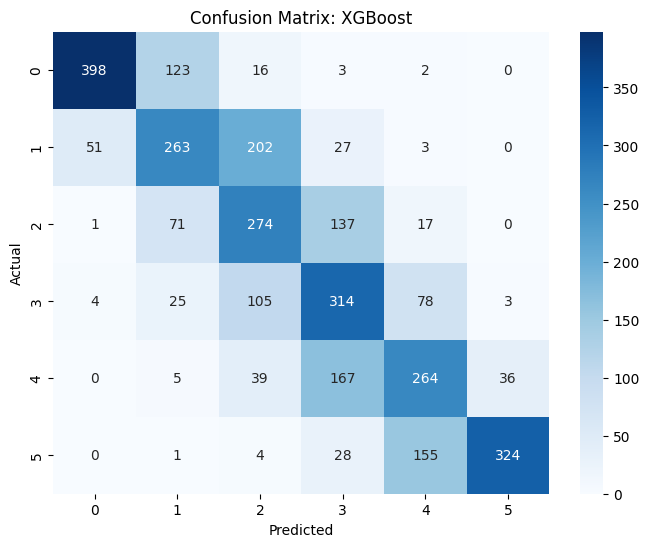
\includegraphics[width=\textwidth]{images/xgb_matrix.png}
    \caption{Best XGB Confusion Matrix}
    \label{fig:xgb_matrix}
\end{subfigure}
\hfill
\begin{subfigure}[b]{0.48\textwidth}
    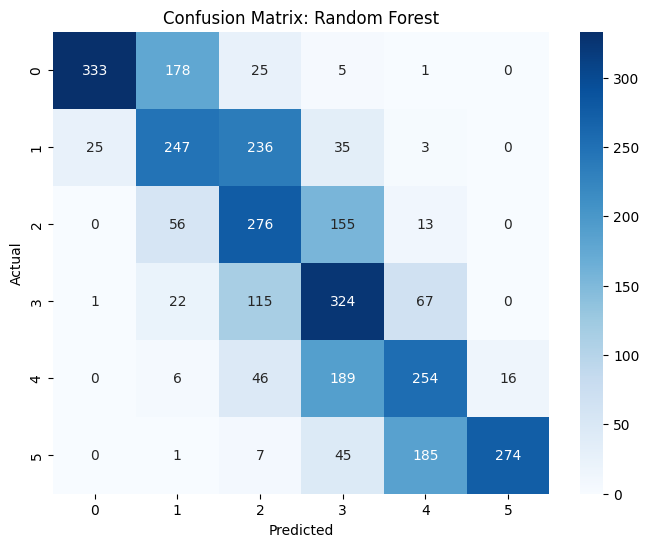
\includegraphics[width=\textwidth]{images/rf_matrix.png}
    \caption{Best RF Confusion Matrix}
    \label{fig:rf_matrix}
\end{subfigure}
\caption{Confusion Matrices for Best Models}
\label{fig:confusion_matrices}
\end{figure}

\noindent \textbf{Random Forest Performance:}
\begin{itemize}
    \item Train RMSE: 0.1056
    \item Test RMSE: 0.8353
\end{itemize}

\noindent \textbf{XGBoost Performance:}
\begin{itemize}
    \item Train RMSE: 0.2268
    \item Test RMSE: 0.7917
\end{itemize}

\subsection{Analysis of Performance}

Although both the Random Forest and XGBoost models exhibited a noticeable gap between training and testing RMSEs, suggesting potential overfitting, these specifically tuned versions outperformed other more generalized configurations of the same models in the Kaggle competition. By optimizing hyperparameters, the tuned Random Forest and XGBoost models were able to effectively capture complex relationships and handle a large number of features, resulting in superior predictive accuracy.

\section{Interpretable Modeling Approaches}

To enhance the interpretability of the models, we employed feature engineering techniques that resulted in easily understandable and logically intuitive features. This approach allows for a clearer understanding of how different variables influence the Airbnb listing prices.

\subsection{Interpretable Feature Engineering Pipeline}

As detailed in the Feature Engineering section, we created new features that encapsulate important aspects of the listings in a manner that is straightforward to interpret. These features were specifically designed to enhance the models' transparency and make the predictive factors easily understandable.

The \texttt{amenities\_count} feature represents the total number of amenities offered by a listing. This aggregated count is highly interpretable, as it directly reflects the number of desirable amenities provided. By summarizing multiple binary features into a single numerical value, it simplifies the evaluation process for decision trees, allowing for a clearer understanding of how the quantity of amenities influences listing prices without introducing unnecessary complexity.

The \texttt{host\_responsiveness} feature combines the host's response time and response rate into a single metric, providing an easily interpretable measure of the host's engagement level. This composite score effectively captures the overall responsiveness of the host, which is a crucial factor for guests and can logically influence the price. By consolidating these two related aspects into one feature, the model can better assess the impact of host behavior on listing prices, enhancing the interpretability of the models' predictions.

\subsection{Feature Importance Analysis}

To identify and explain key predictive factors, we performed a feature importance analysis using both the Random Forest and XGBoost models. This analysis reveals which features have the most significant impact on the models' predictions.

\begin{figure}[H]
\centering
\begin{subfigure}[b]{0.48\textwidth}
    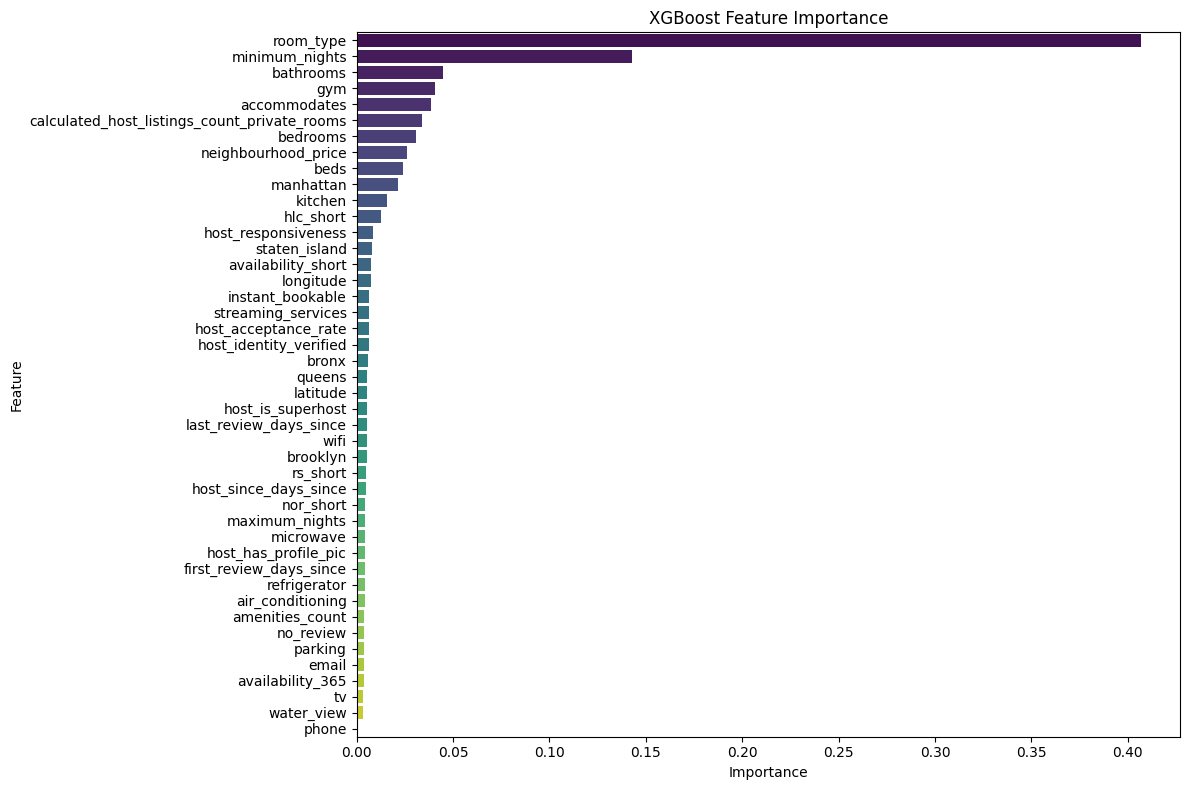
\includegraphics[width=\textwidth]{images/xgb_importance.png}
    \caption{XGBoost Feature Importance}
    \label{fig:xgb_importance}
\end{subfigure}
\hfill
\begin{subfigure}[b]{0.48\textwidth}
    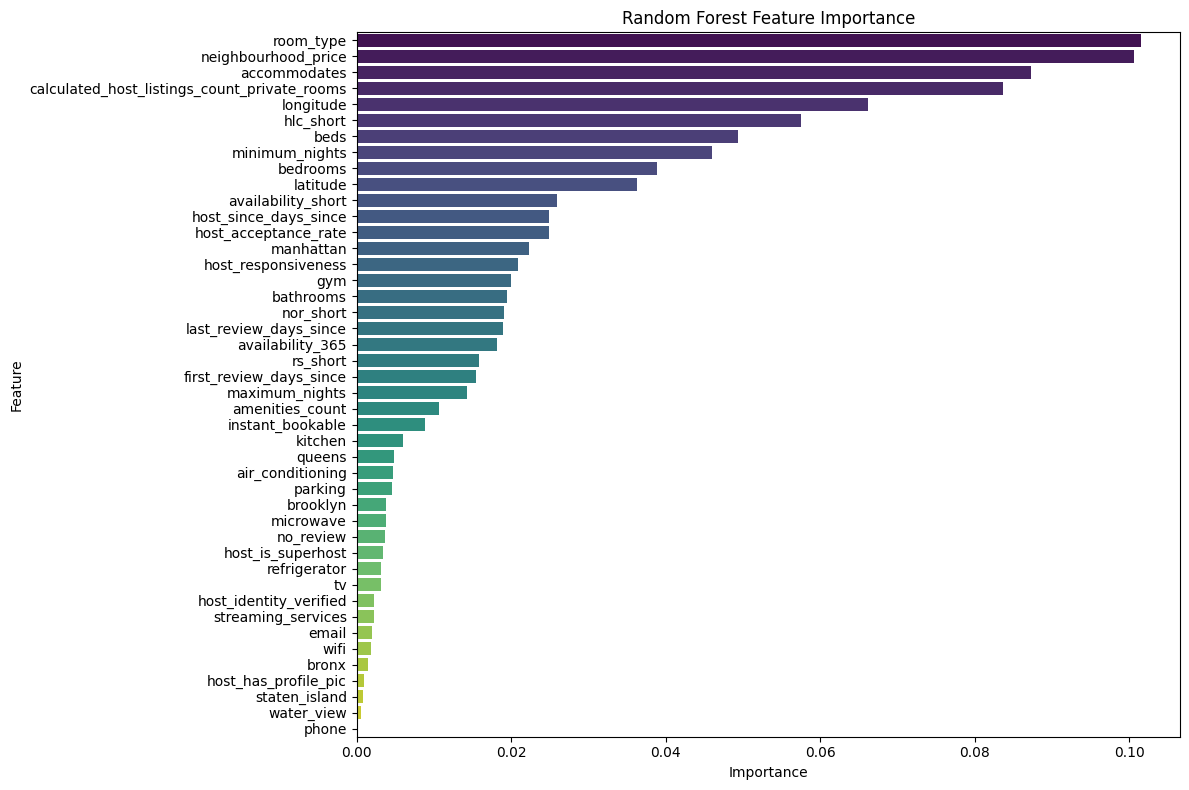
\includegraphics[width=\textwidth]{images/rf_importance.png}
    \caption{Random Forest Feature Importance}
    \label{fig:rf_importance}
\end{subfigure}
\caption{Feature Importance Plots}
\label{fig:feature_importance}
\end{figure}

\subsubsection{Key Predictive Factors}

The feature importance plots in Figure \ref{fig:feature_importance} highlight the most influential features in predicting Airbnb listing prices.

The top features identified by the Random Forest model include:

\begin{itemize}
    \item \texttt{room\_type} (Importance: 0.1015)
    \item \texttt{neighbourhood\_price} (Importance: 0.1006)
    \item \texttt{accommodates} (Importance: 0.0873)
\end{itemize}

Similarly, the XGBoost model identified the following top features:

\begin{itemize}
    \item \texttt{room\_type} (Importance: 0.4067)
    \item \texttt{minimum\_nights} (Importance: 0.1430)
    \item \texttt{bathrooms} (Importance: 0.0449)
\end{itemize}

\subsubsection{Observations on Feature Importance}

It is notable that the \texttt{room\_type} feature is highly influential in the XGBoost model, with an importance score of 0.4067. This indicates that the type of accommodation (e.g., entire home, private room) is a key determinant of listing prices, aligning with intuitive expectations as different room types naturally command varying price ranges.

Conversely, engineered features such as \texttt{water\_view} demonstrated low importance, scoring 0.0005 in the Random Forest model and even lower in XGBoost. Similarly, other amenities like \texttt{wifi} and \texttt{parking} showed minimal impact, suggesting that while these features enhance the overall appeal of a listing, their direct effect on price prediction is overshadowed by more dominant factors.

\subsubsection{Interpretation of Engineered Features}

The engineered features, such as \texttt{amenities\_count} and \texttt{host\_responsiveness}, also appeared in the feature importance rankings, demonstrating their relevance:

\begin{itemize}
    \item \texttt{amenities\_count} had an importance of 0.0107 in the Random Forest model and 0.0041 in the XGBoost model, lower than expected.
    \item \texttt{host\_responsiveness} had an importance of 0.0209 in the Random Forest model and 0.0083 in the XGBoost model, a good result, even outperforming other \texttt{host} features in some cases.
\end{itemize}

These importance scores indicate that the number of amenities and host responsiveness are significant predictors of listing prices. Their interpretability makes it easier to understand how improvements in these areas could potentially increase a property's price.

\subsubsection{Insights Gained}

By analyzing feature importance, we gain valuable insights into what drives the pricing of Airbnb listings:

\begin{itemize}
    \item \textbf{Room Type:} The most critical feature, indicating that the type of accommodation (e.g., entire home, private room) greatly affects the price.
    \item \textbf{Location:} Features like \texttt{neighbourhood\_price}, \texttt{longitude}, and borough indicators (e.g., \texttt{manhattan}, \texttt{brooklyn}) highlight the impact of location.
    \item \textbf{Capacity and Amenities:} Features such as \texttt{accommodates}, \texttt{bathrooms}, and \texttt{amenities\_count} show that larger properties with more amenities command higher prices.
    \item \textbf{Host Factors:} The \texttt{host\_responsiveness} feature underscores the importance of host engagement in pricing.
\end{itemize}

\section{Conclusion}

In conclusion, this project demonstrates the successful application of interpretable machine learning techniques to predict Airbnb rental prices in New York City. By combining robust feature engineering, advanced preprocessing, and hyperparameter optimization using Optuna, we achieved high predictive accuracy, with XGBoost outperforming Random Forest in RMSE on the test set. The analysis also provided clear insights into key drivers of rental pricing, such as room type, neighborhood price indicators, and listing capacity, while engineered features like host responsiveness and amenities count offered added interpretability.


\nocite{*}
\printbibliography

\end{document}